\documentclass[UTF8,AutoFakeBold,AutoFakeSlant,zihao=-4]{ctexart}

\newcommand{\emp}{\noindent\fboxsep=0pt}

\usepackage{wrapfig}
\usepackage{fontspec}
\usepackage{color}
\usepackage{fancyhdr}
\usepackage{setspace}
\usepackage{caption}
\usepackage{mathptmx}
\usepackage{amsmath}
\usepackage{amssymb}
\usepackage{amstext}
\usepackage{geometry}
\usepackage{graphicx}
\usepackage{enumerate}
\usepackage{enumitem}
\usepackage{pifont}
\usepackage{float}
\usepackage{newclude}
\usepackage{subfig}
\usepackage{multirow}
\usepackage{tabularx}
\geometry{
a4paper,
left=2.5cm,
right=2.5cm,
top=2.5cm,
bottom=2.5cm,
}
%\usepackage{listings}
%\usepackage{boxedminipage}

% 设置n倍行距(需要注释掉正文中设置行距的部分)
% \linespread{1.5} % 正文1.5倍行距

%定义一级二级三级标题
\ctexset{
	section = {	% 定义一级标题 
	           	format+ = \zihao{4} \heiti \raggedright, 	% 字号为’四号‘,字体为’黑体‘,左对齐
	           	name = {,、},                             	% 序号后面加’、‘
	           	number = \chinese{section},              	% 序号为’汉字‘
	           	beforeskip = 1.0ex plus 0.2ex minus .2ex,	% 标题前的垂直间距 = 基础高度为1.0ex,可以伸展到 1.0 - 0.2 = 1.2ex,也可以收缩到 1.0 - .2 = 0.8ex; ex为当前字号下字母x的高度
	           	afterskip = 1.0ex plus 0.2ex minus .2ex, 	% 标题后的垂直间距 = ...	
	           	aftername = \hspace{0pt}                 	% 编号和标题之间的格式 = 增加水平间距’0pt‘ 
	},
	subsection = {	% 定义二级标题
	              	format+ = \zihao{-4} \songti \raggedright,
	              	name = {(,)},
	              	number = \chinese{subsection},	% 序号为’阿拉伯数字‘
	              	beforeskip = 1.0ex plus 0.2ex minus .2ex,
	              	afterskip = 1.0ex plus 0.2ex minus .2ex,
	              	aftername = \hspace{0pt},
	},
	subsubsection = {
			format+ = \zihao{-4} \songti \raggedright,
			name = {\qquad,\ \enspace},
			number = {\arabic{section}.\arabic{subsection}.\arabic{subsubsection}},	
			beforeskip = 1.0ex plus 0.2ex minus .2ex,
			afterskip = 1.0ex plus 0.2ex minus .2ex,
			aftername = \hspace{0pt},
	}
}

% 设置页眉页码
\pagestyle{plain} % 取消页眉
\lfoot{}	% 页码出现在下方

% 定义正文字体
\setromanfont{Times New Roman}	% 将西文字体设置为 Times New Roman
% \setCJKfamilyfont{zhkai}{[SIMKAI.TTF]}
% \newcommand*{\kaiti}{\CJKfamily{zhkai}}

% 定义 caption
\DeclareCaptionFont{kaiticaption}{\kaishu \small}	% 定义下面三个caption的font的kaiticaption的具体格式
\captionsetup[figure]{font=small,labelsep=quad,skip=0.5ex,labelfont=bf,font=kaiticaption}	% 设置图片的 caption 格式 % 想要标题换行后居中,可以添加justification=centering
\captionsetup[table]{font=small,labelsep=quad,skip=0.5ex,labelfont=bf,font=kaiticaption}	% 设置表格的 caption 格式
\captionsetup[subfloat]{font=small,labelsep=quad,skip=0.5ex,labelfont=bf,font=kaiticaption}
\captionsetup[equation]{font=small,labelsep=quad,skip=0.5ex,labelfont=bf,font=kaiticaption}


% 设置图片,表格,公式编号格式
\renewcommand{\thetable}{\thesection{}-\arabic{table}}	% \thetable 表示设置的是表格的编号格式, 后面括号的内容为编号格式:章节号-表格的序号
\renewcommand{\thefigure}{\thesection{}-\arabic{figure}}
\renewcommand{\theequation}{\thesection{}-\arabic{equation}}

% 设置列表标签
\setlist[enumerate]{nosep,itemindent=0.75em,labelsep=0.5em}	% labelsep 是标签与标签后面内容的间距(这里是一个空格),leftmargin是标签后面内容与左边界之间的距离
\setlist[itemize]{nosep,itemindent=0.5em, labelsep=0.5em}
\setlist[description]{nosep,leftmargin=*}
\let\olddescriptionlabel\descriptionlabel  
\renewcommand{\descriptionlabel}[1]{\hspace{2em}\olddescriptionlabel{#1}:}  


% 设置代码块
%\definecolor{commentcolor}{RGB}{85,139,78}
%\definecolor{stringcolor}{RGB}{206,145,108}
%\definecolor{keywordcolor}{RGB}{34,34,250}
%\lstset{
%	language=Matlab, % 默认代码语言.
%	basicstyle=\footnotesize,
%	numbers=left, %设置行号位置
%	numberstyle=\tiny, %设置行号大小
%	commentstyle=\color{commentcolor},	%注释颜色
%	keywordstyle=\color{keywordcolor},	%关键词颜色
%	stringstyle=\color{stringcolor},	%字符串颜色
%	frame=single, %设置边框格式
%	escapeinside=``, %逃逸字符(1左面的键),用于显示中文
%	breaklines = True, % 自动折行
%	breakatwhitespace = True, % 自动折行时打断单词
%	extendedchars=false, %解决代码跨页时,章节标题,页眉等汉字不显示的问题
%	xleftmargin=2em,xrightmargin=2em, aboveskip=1em, %设置边距
%	tabsize=4, %设置tab空格数
%	showspaces=false %不显示空格
%}

\graphicspath{{../img/}}
\title{车身电气}
\author{}
\date{}
\begin{document}
\setlength{\parskip}{0em}	% 段前段后间距为 0
\setlength{\parindent}{2em} % 正文首行悬挂: 2汉字字符
\setlength{\baselineskip}{20pt}	% 正文行间距20磅
\selectfont	% 刷新行间距信息
\setlength{\lineskip}{10pt}		% 推荐设置为行距的一半
\setlength{\lineskiplimit}{10pt}	% 同上
\abovedisplayshortskip=0pt	%设置公式距离上方非重叠区域额外添加的距离,推荐0
\belowdisplayshortskip=0pt
\abovedisplayskip=0pt	%设置公式距离上方重叠距离额外添加的距离,推荐0
\belowdisplayskip=0pt
\renewcommand{\arraystretch}{1.5}

\maketitle
\section{电气概述}
汽车电气系统由电源系统和用电系统组成

\section{发动机电气系统}
\subsection{启动系统}
	包括:蓄电池、点火开关(启动开关)、启动机总成、起动机继电器
	\begin{figure}[htbp]
		\centering
		\subfloat[启动系统]{\centering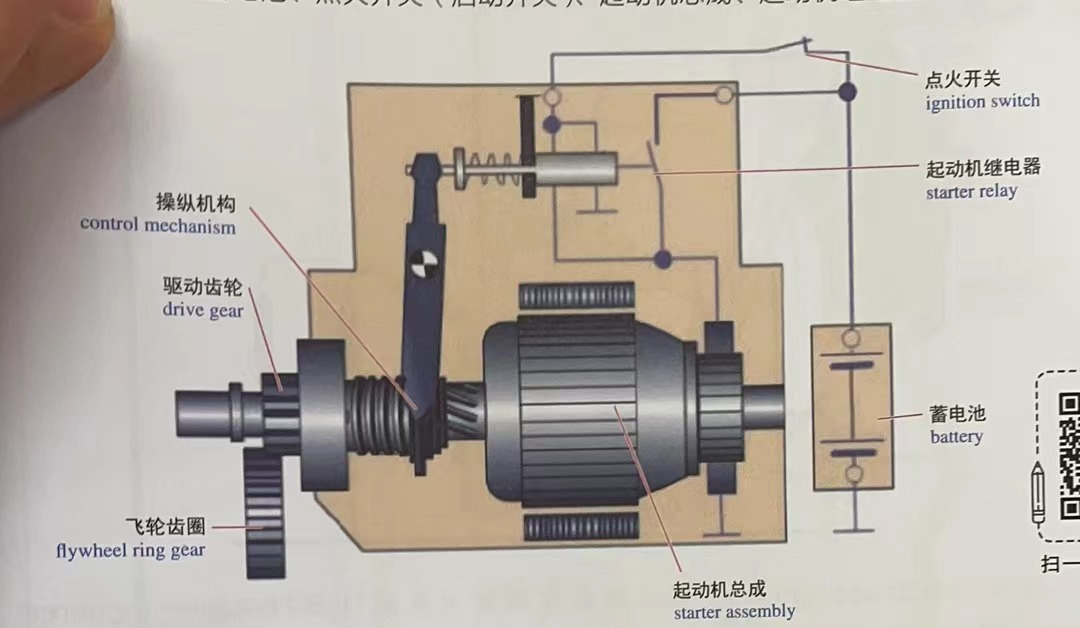
\includegraphics[width=0.5\textwidth]{5-1}}
		\subfloat[启动机示意图]{\centering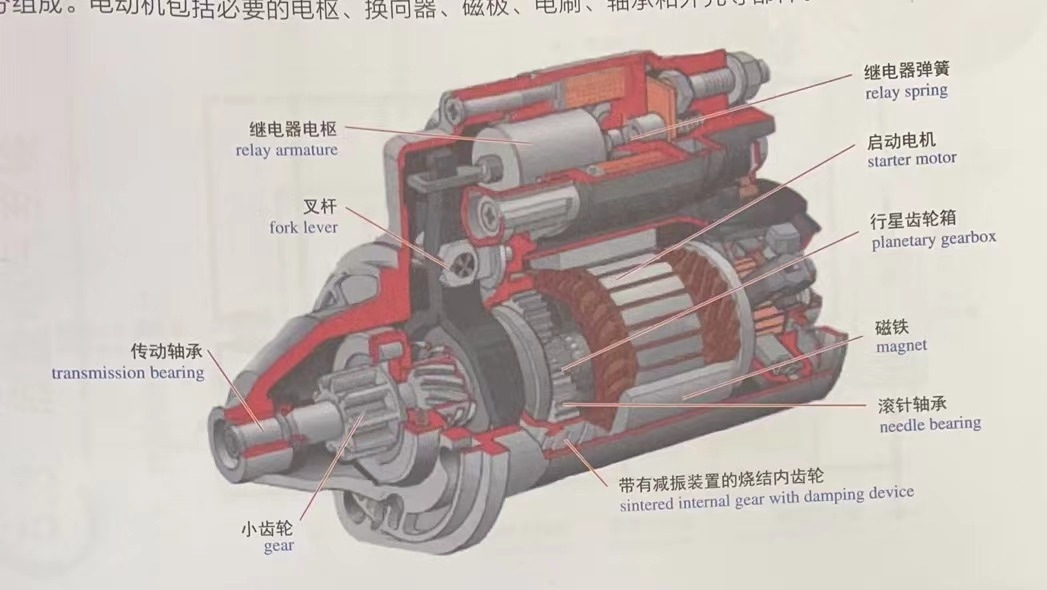
\includegraphics[width=0.5\textwidth]{5-2}}
	\end{figure}
	
	
	蓄电池给启动机内的直流电机供电,启动机带动发动机飞轮转动 through 传动机构,发动机启动
\subsection{点火系统}
	点火系统用于按次序使火花塞产生电火花
	\subsubsection{机械式点火系统}
		曲轴带动分电器轴转动,分电器轴的凸轮使点火线圈初级触点闭合产生高压电,高压电通过分电器轴上的分火头达到指定的火花塞,火花塞发出电火花
	\subsubsection{电子点火系统}
		分为:晶体管点火系统TI-B、半导体点火系统SI、无分电器点火系统DIS(每一缸都有专用的点火线圈,由ECU控制)
		\begin{figure}[htbp]
			\centering
			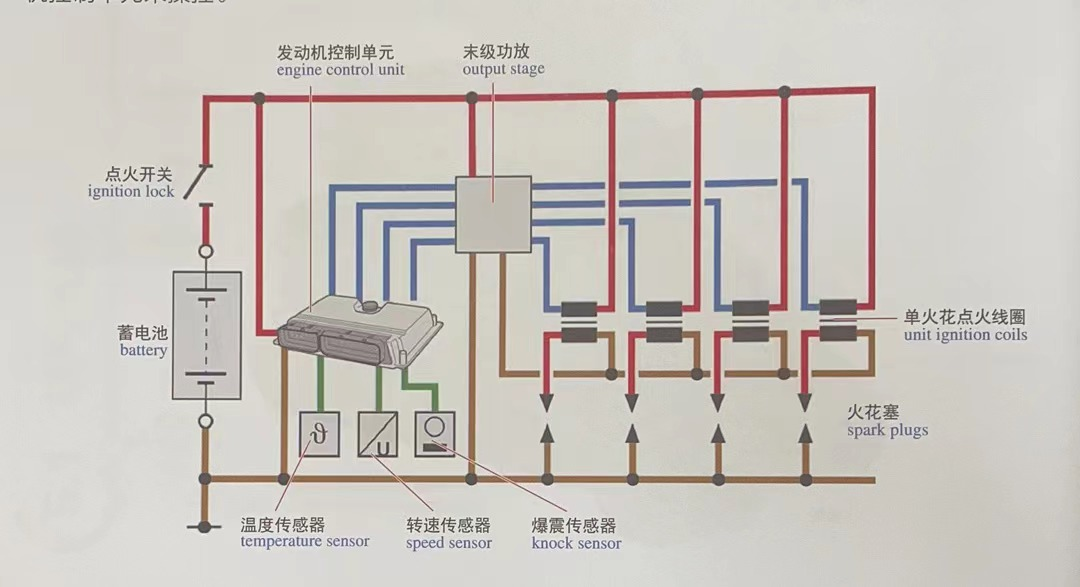
\includegraphics[width=0.5\textwidth]{5-3}
		\end{figure}

\section{底盘电气系统}
\subsection{防抱死制动系统(ABS, anti-locked braking system)}
	\subsubsection{componnents}
		ECU、轮速传感器、制动压力调节装置和制动控制电路
		\begin{figure}[htbp]
			\centering
			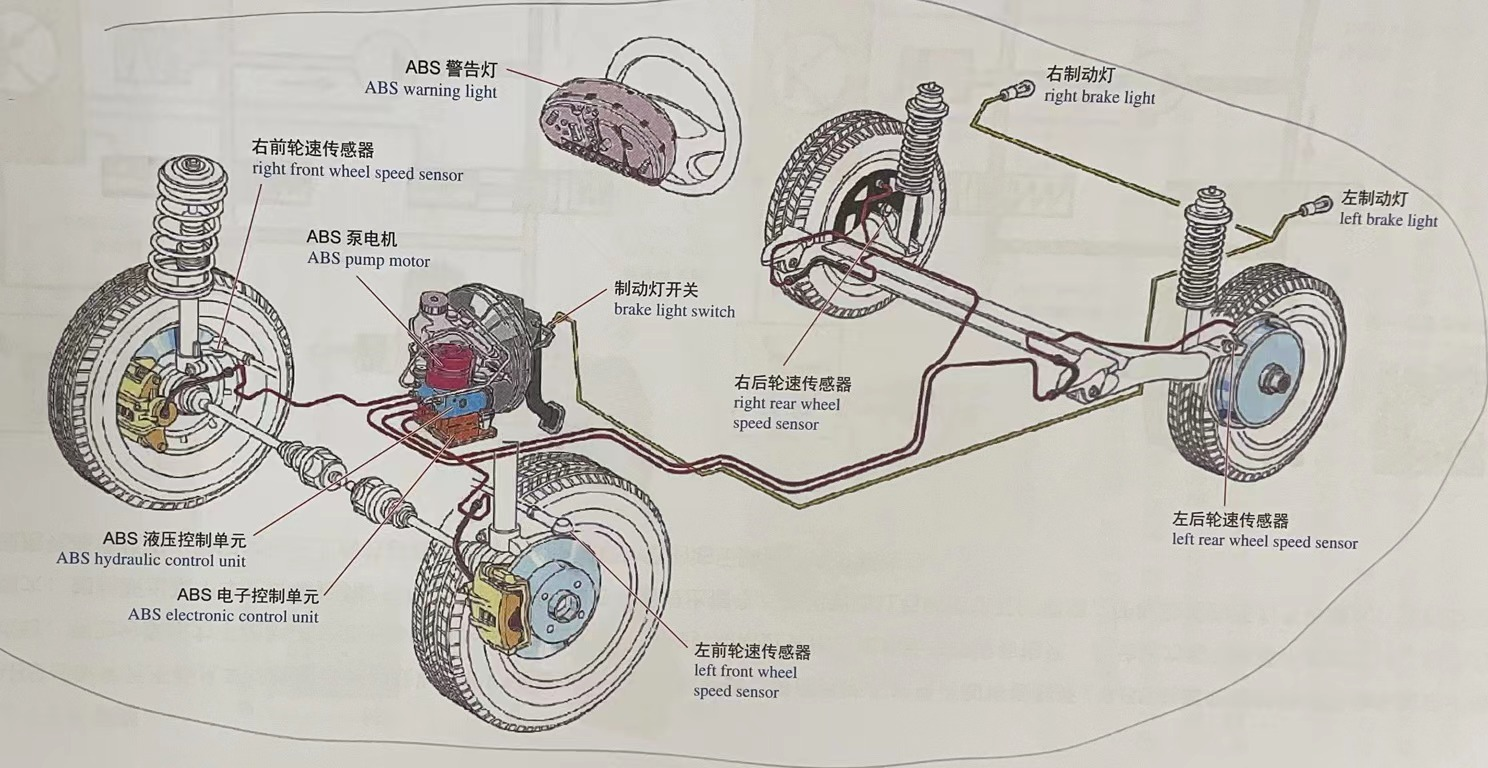
\includegraphics[width=0.5\textwidth]{5-4}
		\end{figure}
	\subsubsection{原理}
		如果ECU判断出车轮没抱死,制动压力调节装置不工作,制动力继续增大
		
		如判断出即将抱死,ECU向制动压力调节装置发出指令,~关闭制动缸和制动轮缸的通道,制动力不再增大
		
		如判断出抱死拖滑,ECU向制动压力调节装置发出指令,使制动轮缸油压降低,减少制动力
\subsection{行驶稳定系统(ESP, electronic stability program)}
	\begin{figure}[htbp]
		\centering
		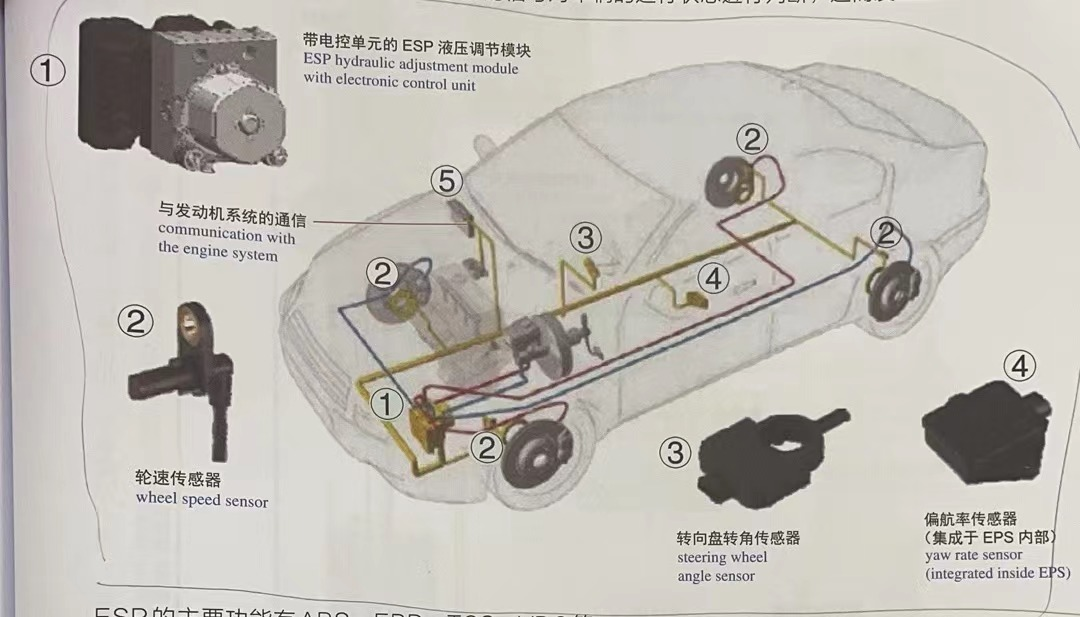
\includegraphics[width=0.5\textwidth]{5-5}
	\end{figure}
	是博世公司为提高行车的主动安全性而发明的牵引力/制动力控制系统
	
	电子稳定控制系统(ESC)、车身稳定控制系统(VSC)之流相当于是换名的ESP
	\subsubsection{组成}
		控制总成、转向传感器(监测转向盘的转向角度)、轮速传感器、侧滑传感器(监测车体绕纵轴转动的状态)、横向加速度传感器(检测汽车转弯时的离心力)……
		
		ECU通过这些传感器的信号对车辆的运行状态进行判断,进而发出控制命
	\subsubsection{功能}
		\begin{enumerate}
			\item  ABS
			\item  EBD电子制动力分配系统
			\item  TCS牵引力控制系统
			\item  VDC主动横摆控制系统
			\item  HBA液压制动器辅助
			\item  HHC上坡辅助
			\item  CDP针对于驻车制动的减速度控制
			\item  HDC陡坡缓降
			\item  AVH自动驻车
		\end{enumerate}
	
\subsection{转向系统}
	包括“电控转向系统”,“动态转向系统”,“全轮转向系统”
	
\subsection{电控转向系统}
	种类:电控液压助力系统、电动电动助力系统
	\begin{center}
		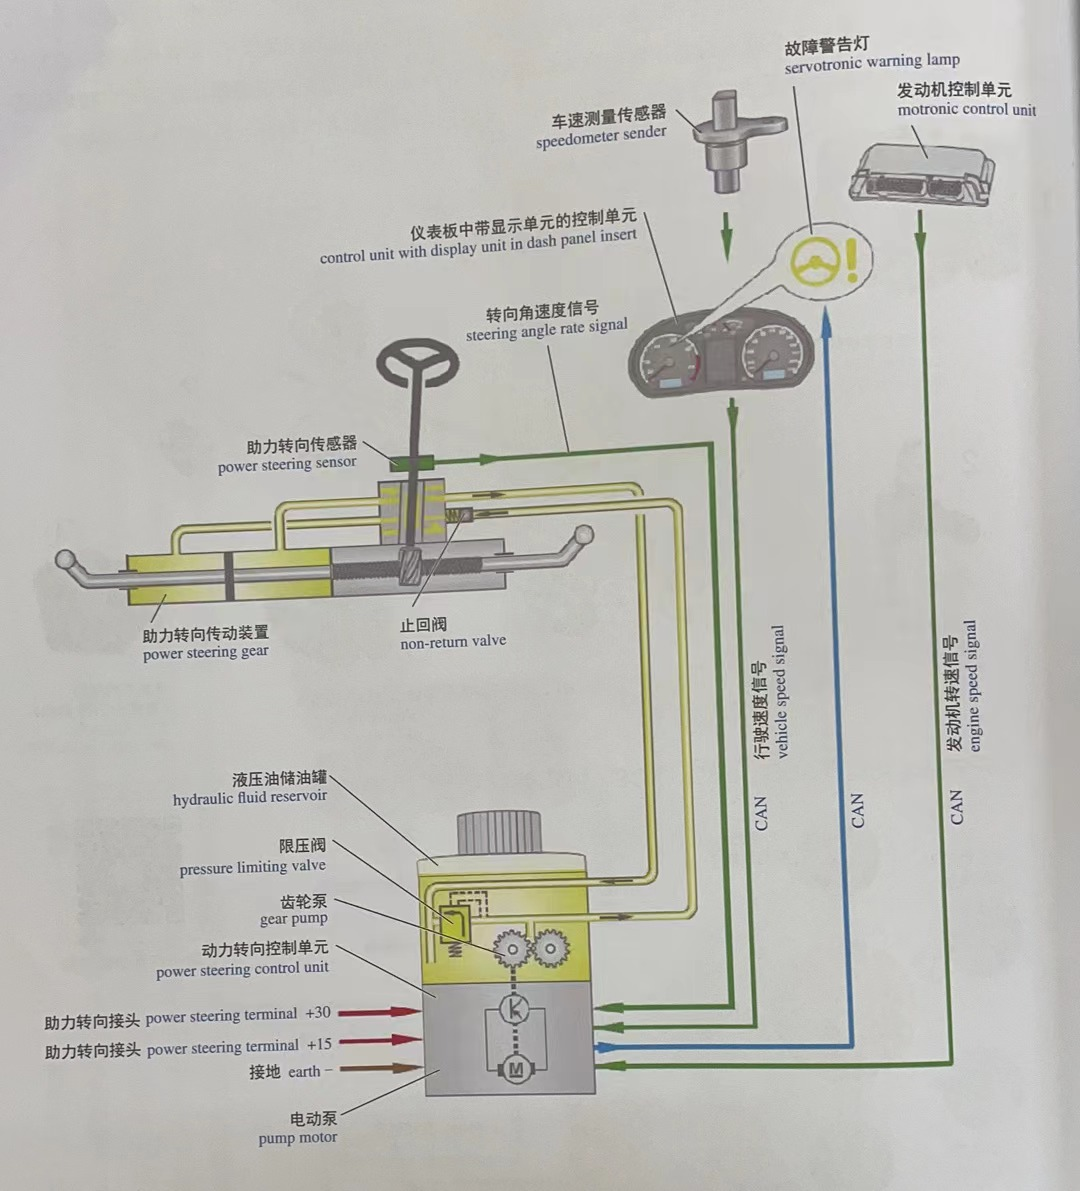
\includegraphics[width=0.45\textwidth]{5-6}
	\end{center}

	\subsubsection{电控液压助力系统}
		\begin{itemize}
			\item  助力转向控制单元集成在电动泵总成中,根据转向角速度和车辆行驶速度发出信号,驱动齿轮泵
			
			\item  瞬时供油量 be read from 通用特性图 saved in ECU
			
			\item  助力转向传感器安装在助力转向装置的分流阀内,提供转向角和转向角速度
			
			\item   转向角传感器安装在转向臂和转向轮之间的转向柱上
			
			\item  ABS传输转向角信号 to 转向轮 in CAN总线,转向轮被驱动
		\end{itemize}
		\begin{figure}[htbp]
			\centering
			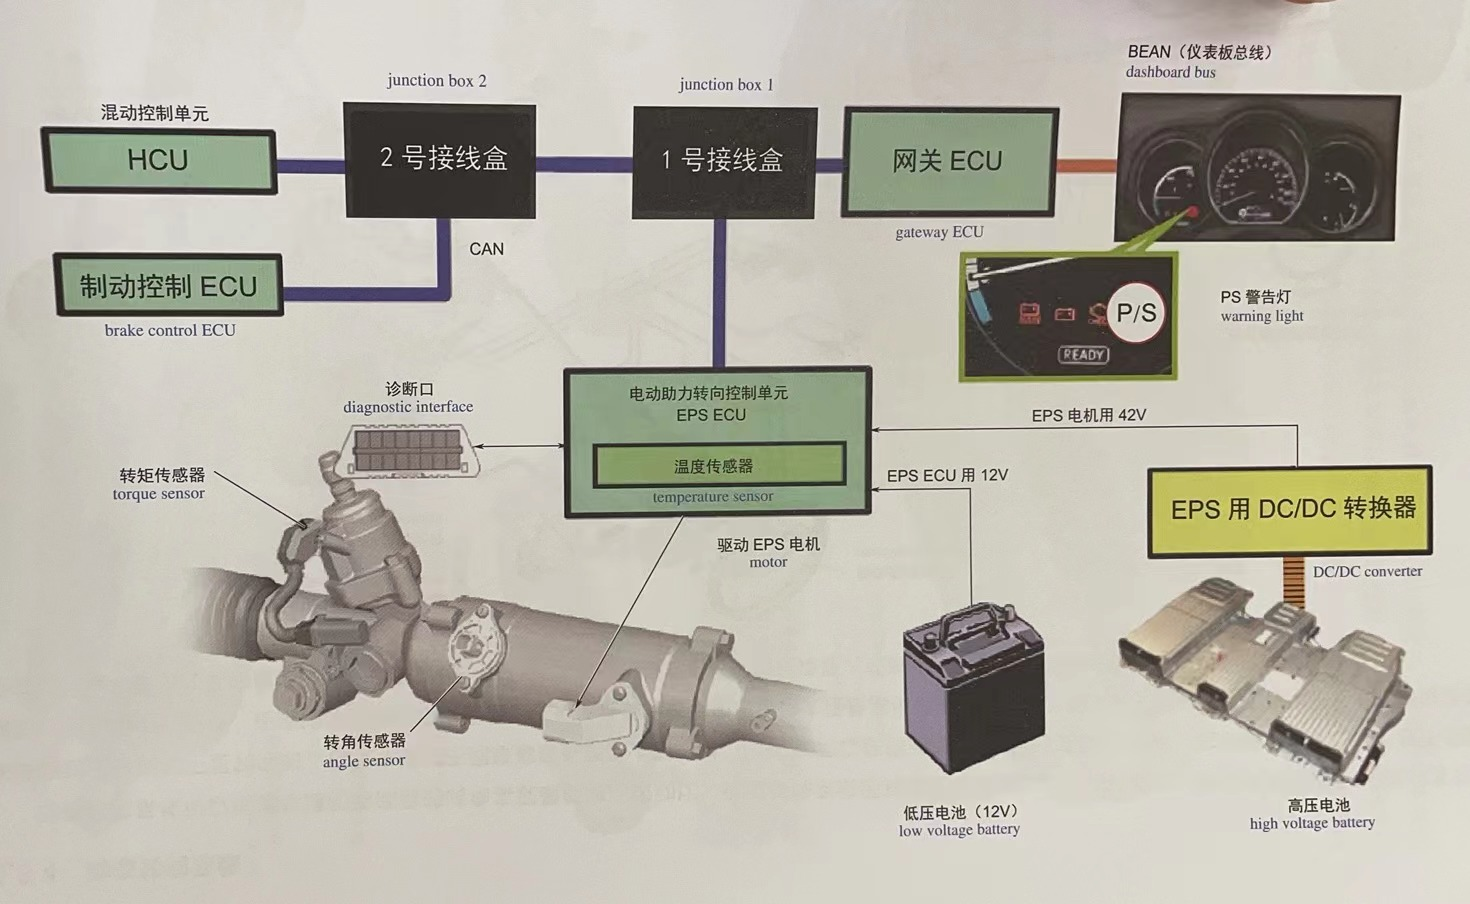
\includegraphics[width=0.5\textwidth]{5-7}
		\end{figure}
	
	\subsubsection{电动助力转向系统EPS}
		组成:转矩穿传感器、电子控制单元、ECU和助力电机
		
		原理:各传感器传输信号到电子控制单元,电控单元计算所需的转向助力 and 通过功率放大模块控制助力电机的转动,助力电机带动减速机构(可以降速增矩),减速机构带动齿轮齿条机构,齿轮齿条机构输出转向助力
		
\subsection{动态转向系统}
	可根据车速和转向盘的转角实现最佳的转向传动比
	
	车轮总转向角 = 司机的转向角 + 并行转角(控制器计算出要额外提供的转向角(并行转角),在操纵一个电机驱动并行转向机提供该转角)
	\begin{figure}[htbp]
		\centering
		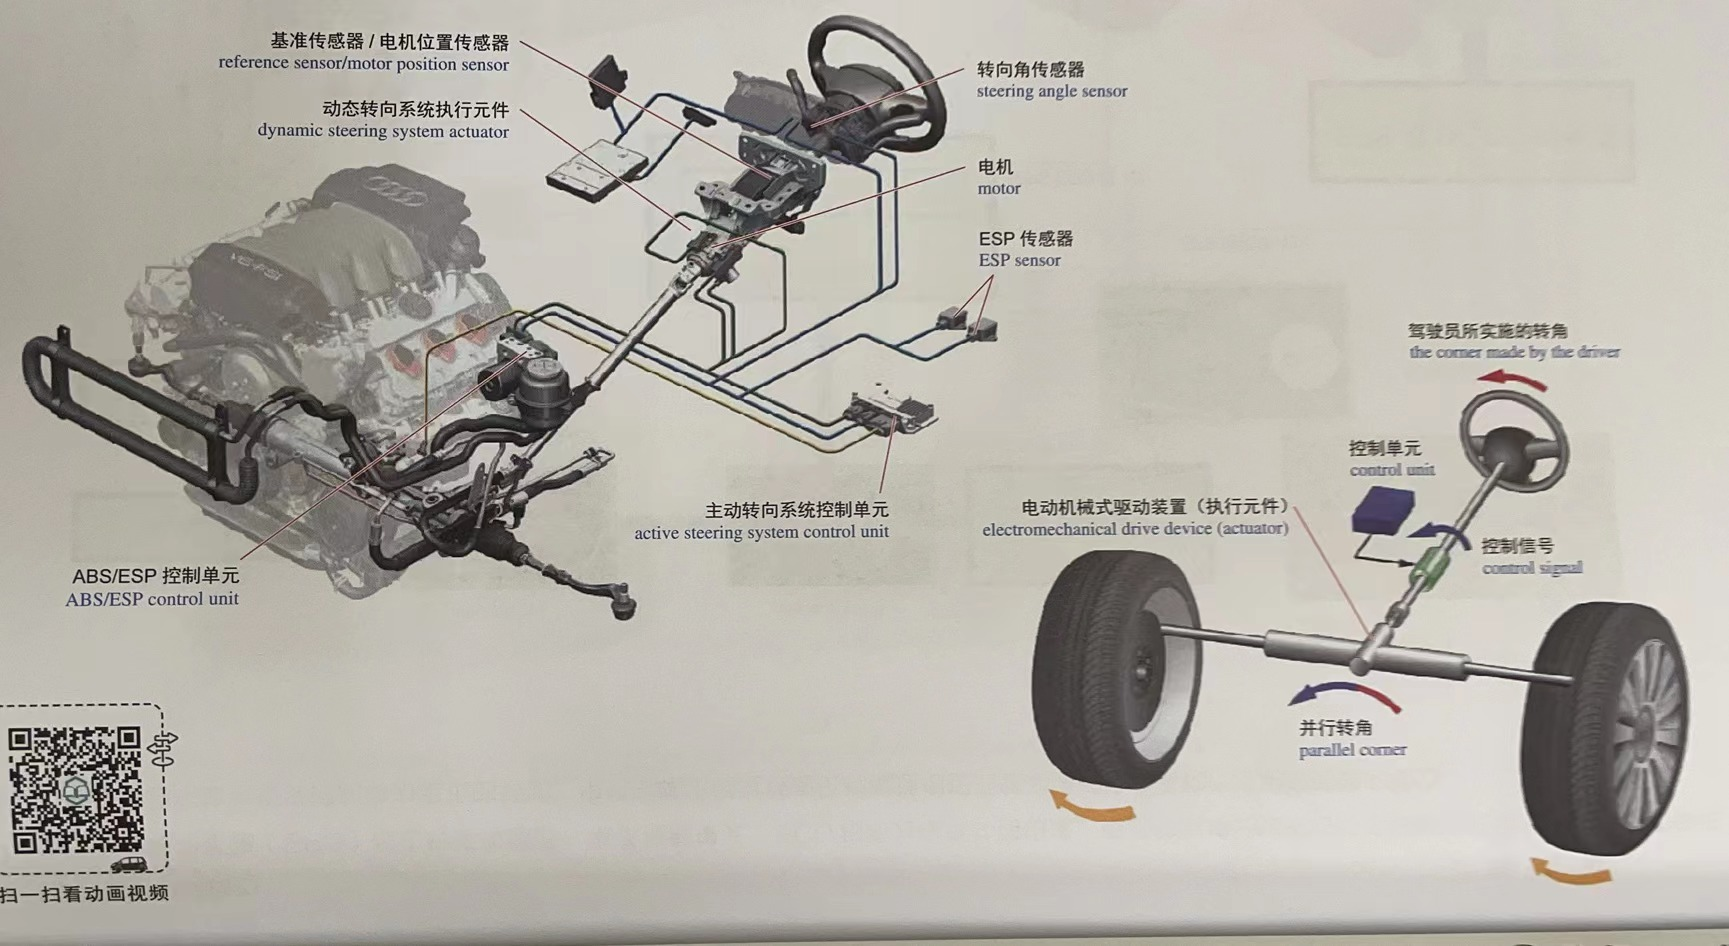
\includegraphics[width=0.5\textwidth]{5-8}
	\end{figure}

\subsection{全轮转向系统}
	就是在EPS的基础上添加了动态转向系统和后轮转向系统。
	
	前后轮所需的转向角都由底盘控制单(转向助力控制单元、后轮转向控制单元、动态转向控制单元)计算
	\begin{figure}[htbp]
		\centering
		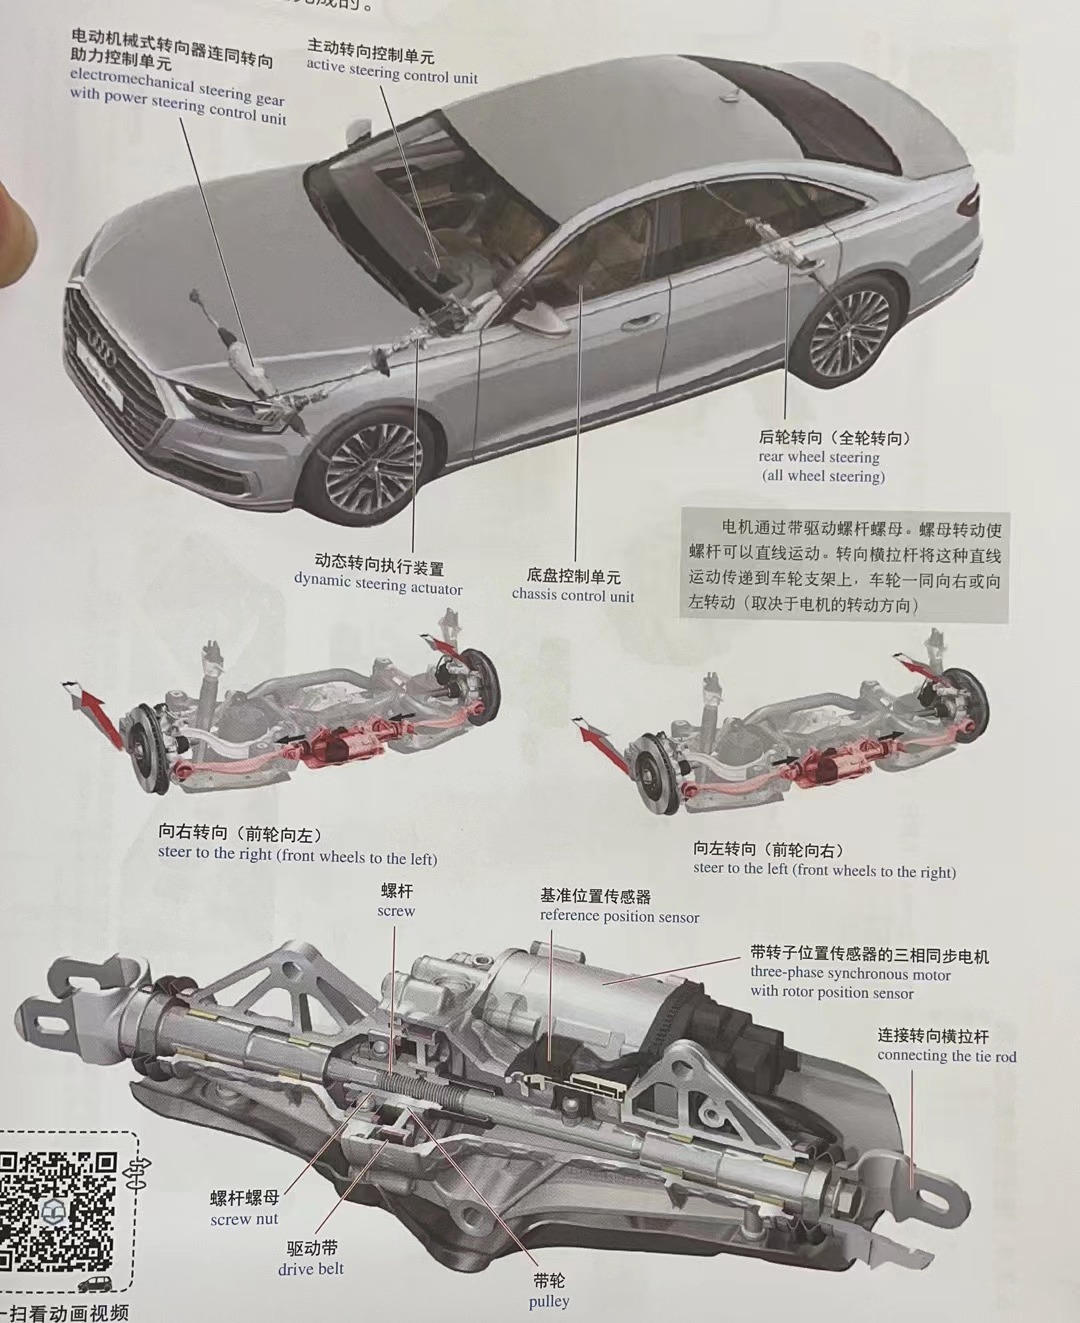
\includegraphics[width=0.5\textwidth]{5-9}
	\end{figure}

\subsection{电子驻车制动系统EPB(electrical park brake)}
	也称“电子手刹”。
	\begin{figure}[htbp]
		\centering
		\caption*{系统结构图}
		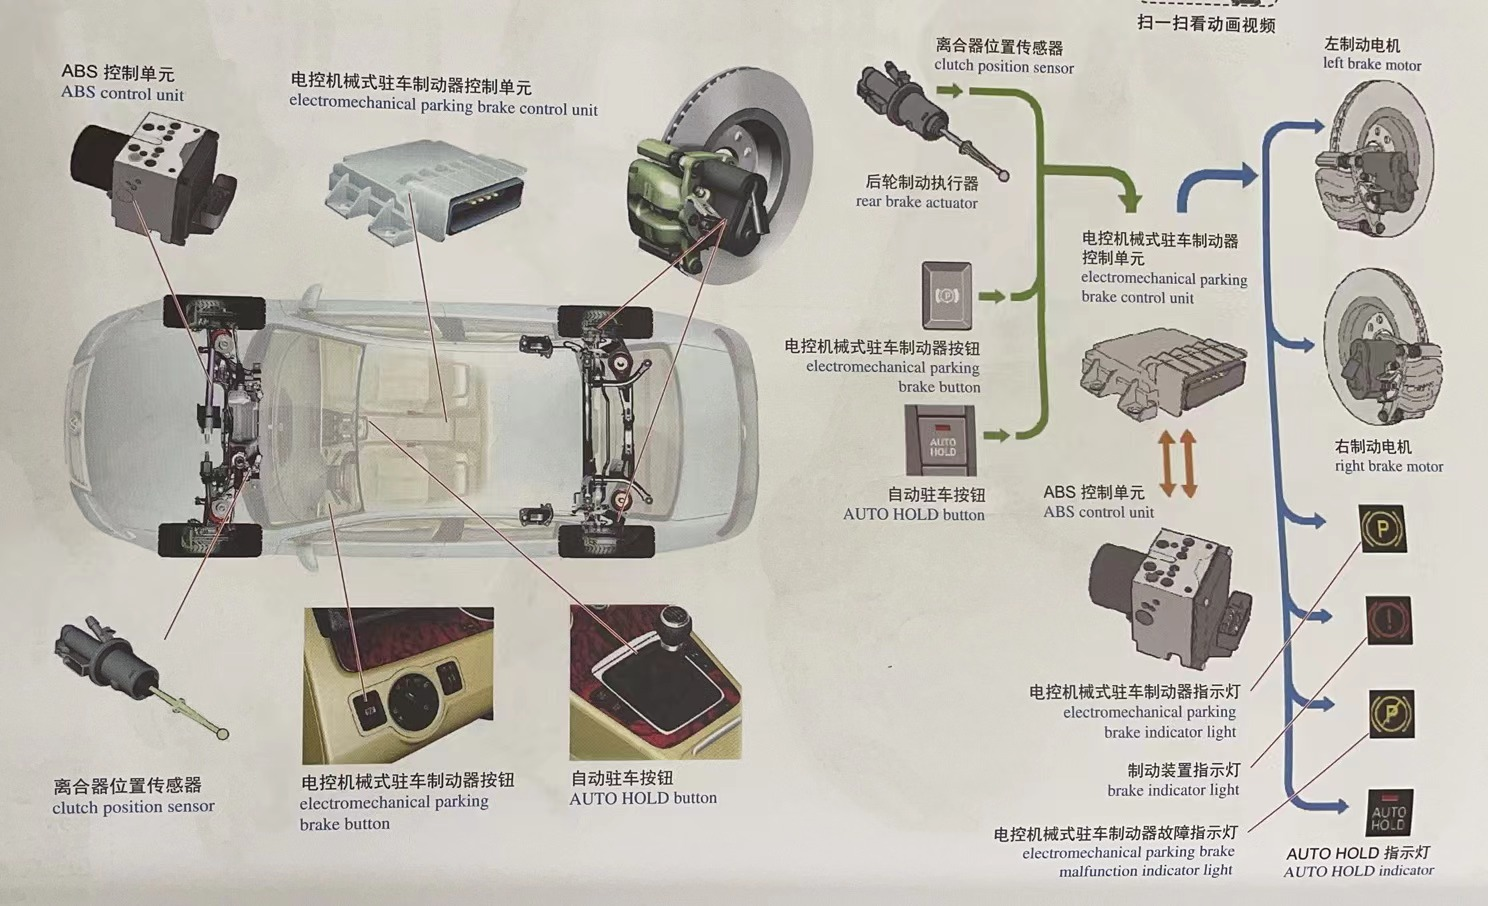
\includegraphics[width=0.5\textwidth]{5-10}
	\end{figure}
	\begin{figure}[htbp]
		\centering
		\caption*{驻车制动器结构图}
		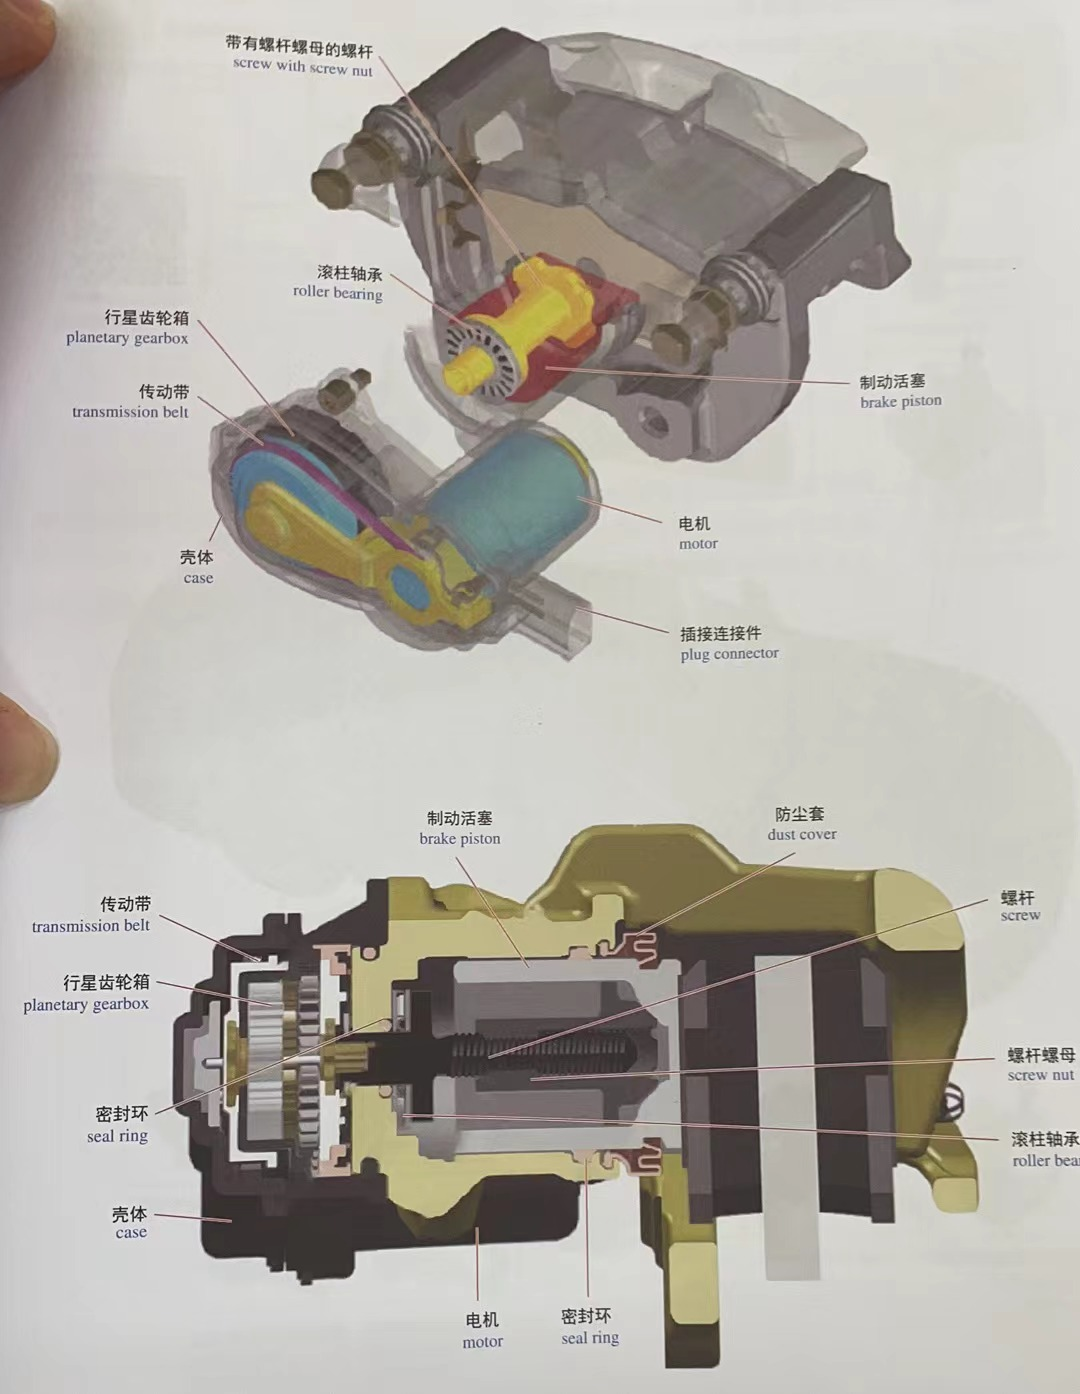
\includegraphics[width=0.5\textwidth]{5-11}
	\end{figure}
\subsection{胎压监测系统}
	\subsubsection{间接胎压监测系统RPA}
		不直接检测轮胎充气压力
		
		过程:胎压下降时,车轮滚动周长变化,从而转速发生变化,车轮轮速传感器向动态稳定控制系统DSC发出信号。当车速超过25km/h和压力下降约30%,组合仪表的指示灯亮起
	\subsubsection{直接胎压监测系统TPMS(tire pressure monitoring system)}
		作用:利用胎压传感器实时监测胎压,对低压和漏气进行警报
		\begin{figure}[htbp]
			\centering
			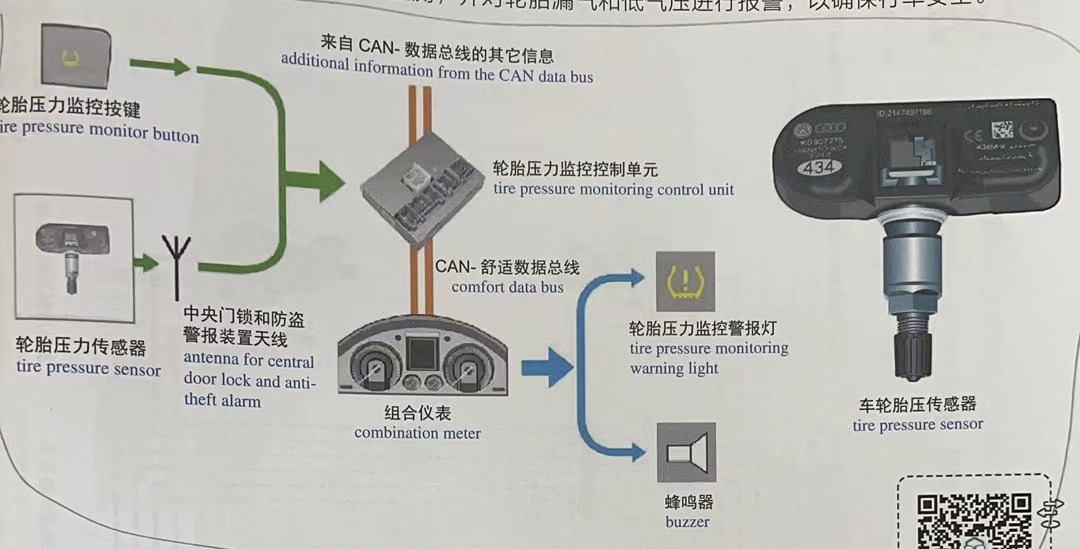
\includegraphics[width=0.5\textwidth]{5-12}
		\end{figure}
\subsection{电子悬架系统EDC}
	\subsubsection{组成}
		\begin{enumerate}
			\item 带有两个调节阀的四个电动调节式减振器
			
			\item 垂直动态管理平台VDP控制单元
			
			\item 四个车辆高度传感器(监测轮胎移动)
			
			\item 探测车身移动(提升、俯仰、侧倾)的传感器
		\end{enumerate}
	\subsubsection{系统}
		\begin{figure}[htbp]
			\centering
			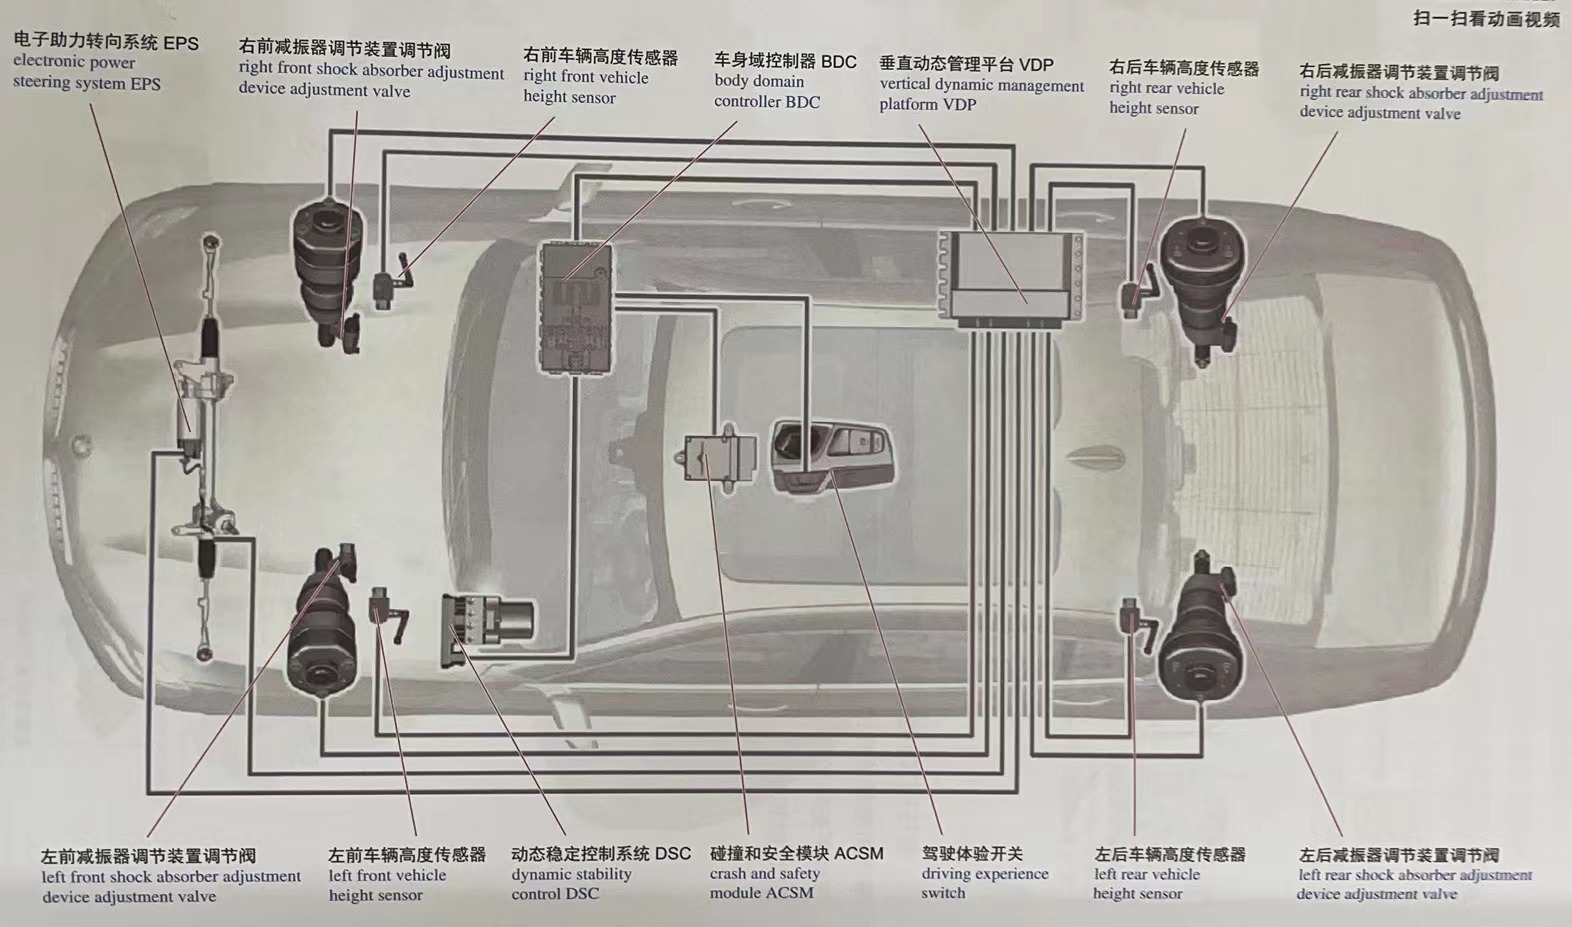
\includegraphics[width=0.5\textwidth]{5-13}
		\end{figure}
\subsection{电子稳定杆系统}
	主动式侧倾稳定杆控制单元(EARSV、EARSH)读取并接受垂直动态管理平台VDP的电码,通过控制电机使各自的稳定杆发生相对扭转,迅速抵消出现的侧倾力矩
	\begin{figure}[htbp]
		\centering
		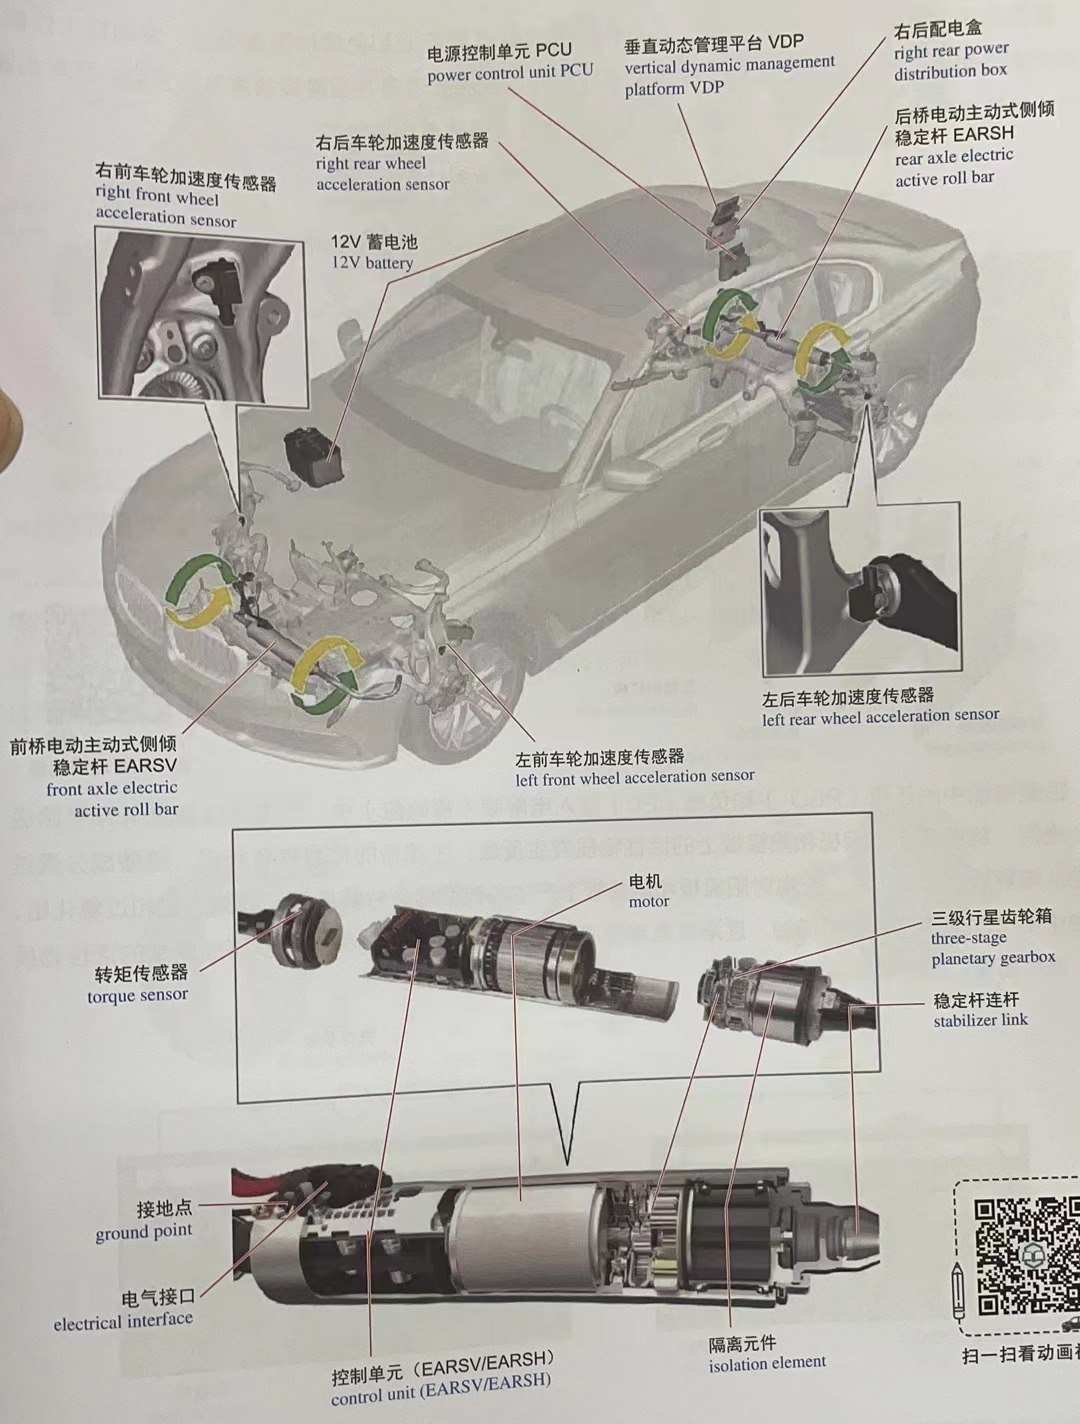
\includegraphics[width=0.5\textwidth]{5-14}
	\end{figure}

\section{车身电气系统}
\subsection{电源系统}
	\begin{enumerate}
		\item 蓄电池
		
		\item 发电机:向用电设备和蓄电池供电
			\begin{figure}[htbp]
				\centering
				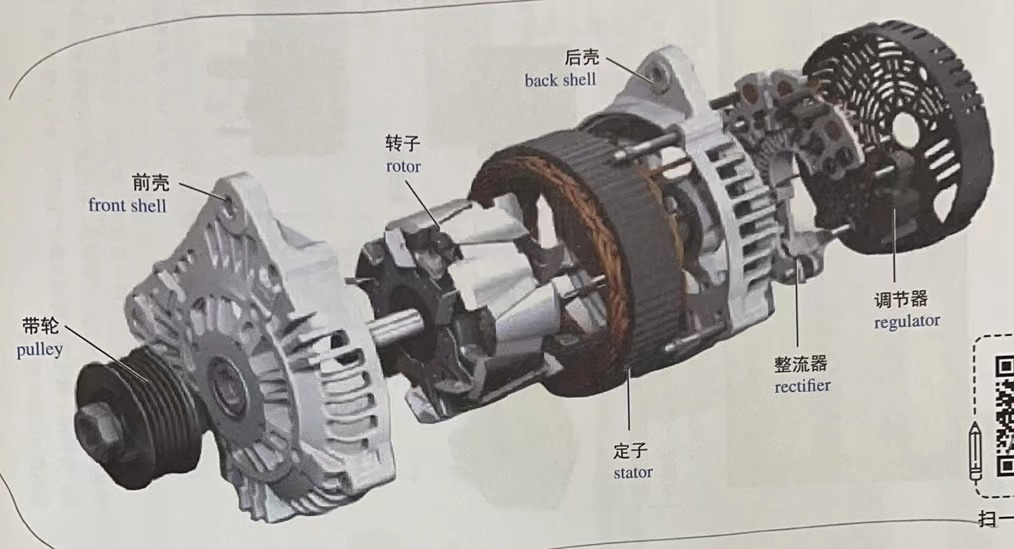
\includegraphics[width=0.5\textwidth]{5-15}
			\end{figure}
			
		\item 配电盒:内置配电系统,包括中央接线盒、电路开关(主要是继电器,有常开型、常闭型、常开常闭混合型)、保险装置(保险丝)、插接件和导线。作用为接受充电及转换的电能以及存储在蓄电池中的电能,再按需分配给其他用电器
			\begin{figure}[htbp]
				\centering
				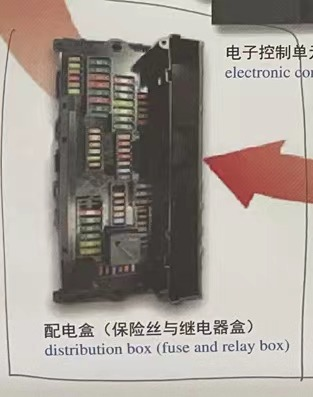
\includegraphics[width=0.25\textwidth]{5-16}
			\end{figure}
	\end{enumerate}

\subsection{照明系统}
	车灯分为照明灯和信号灯。
	\begin{center}
		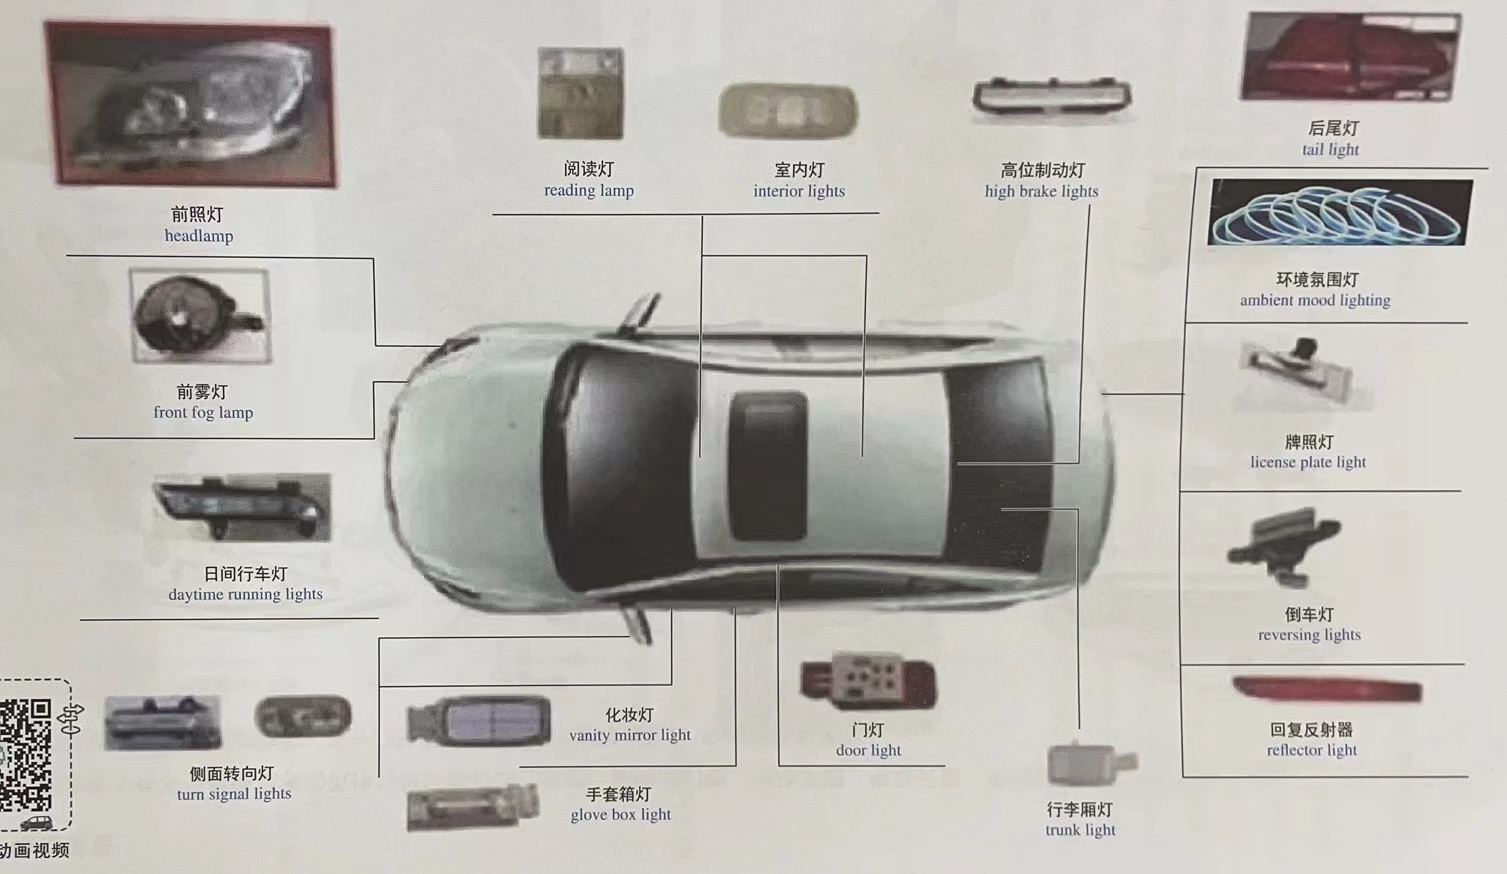
\includegraphics[width=0.5\textwidth]{5-17}
	\end{center}

\subsection{电动装置}
	\begin{figure}[htbp]
		\centering
		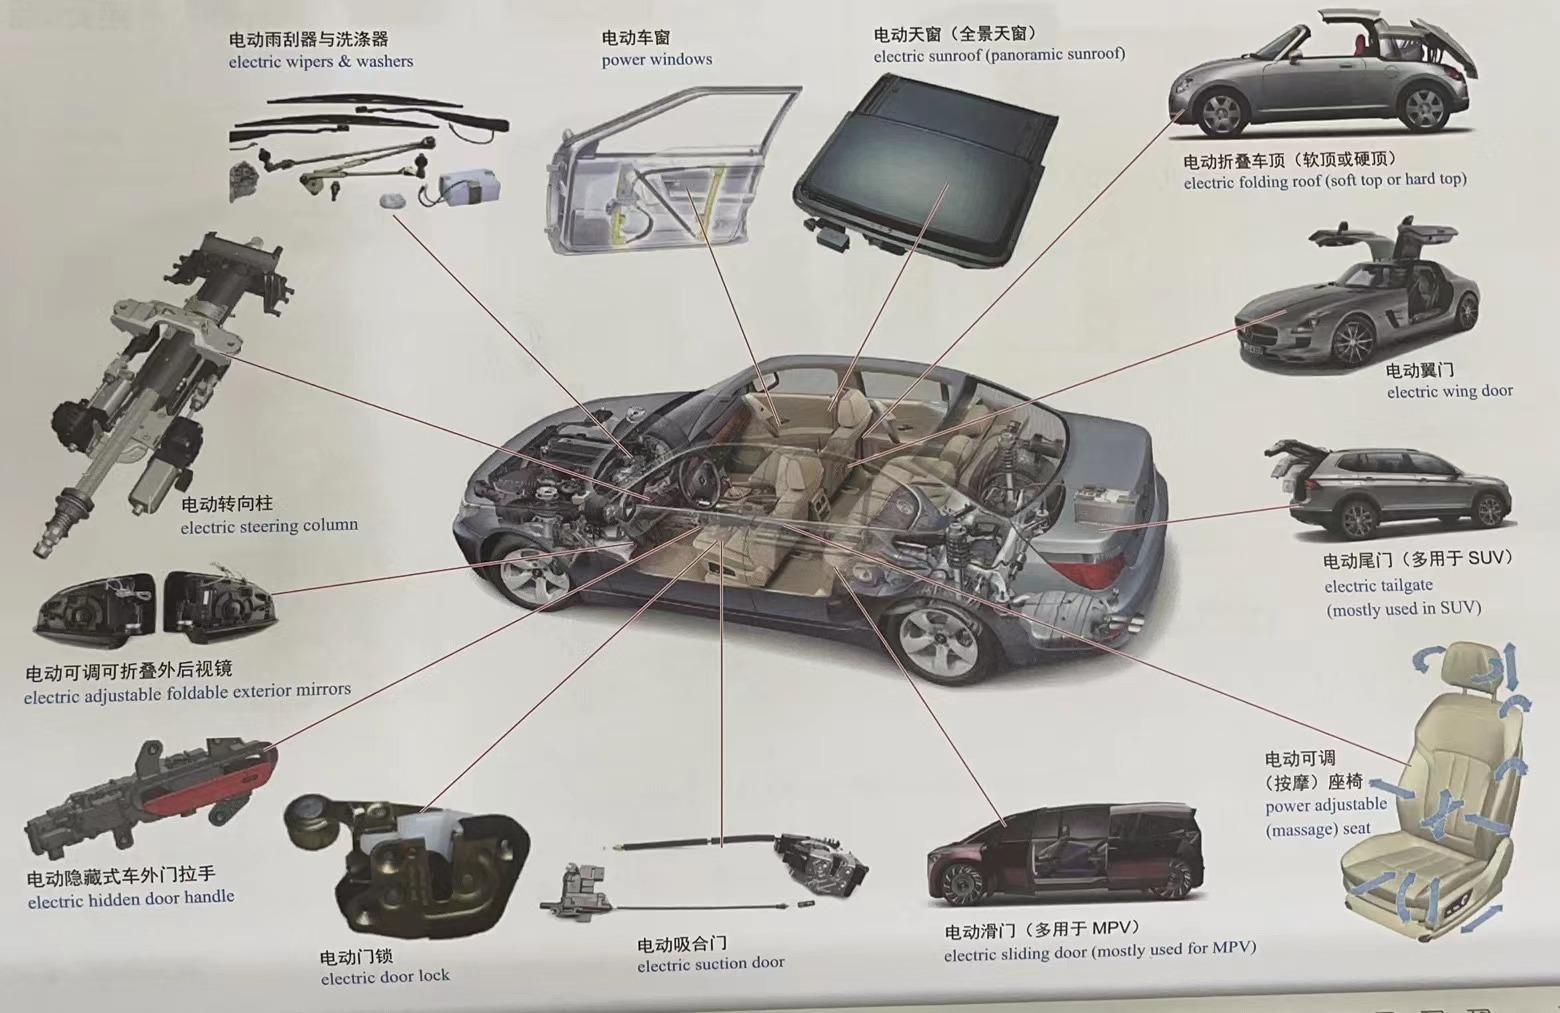
\includegraphics[width=0.5\textwidth]{5-18}
	\end{figure}

\subsection{电热装置}
	常见的有:后风窗除霜器、点烟器、座椅加热器

\subsection{电声装置}
	用来完成电信号和声音信号的转换装置,包括扬声器、鸣笛
	
\subsection{空调系统}
	\subsubsection{燃油车空调}
		\begin{center}
			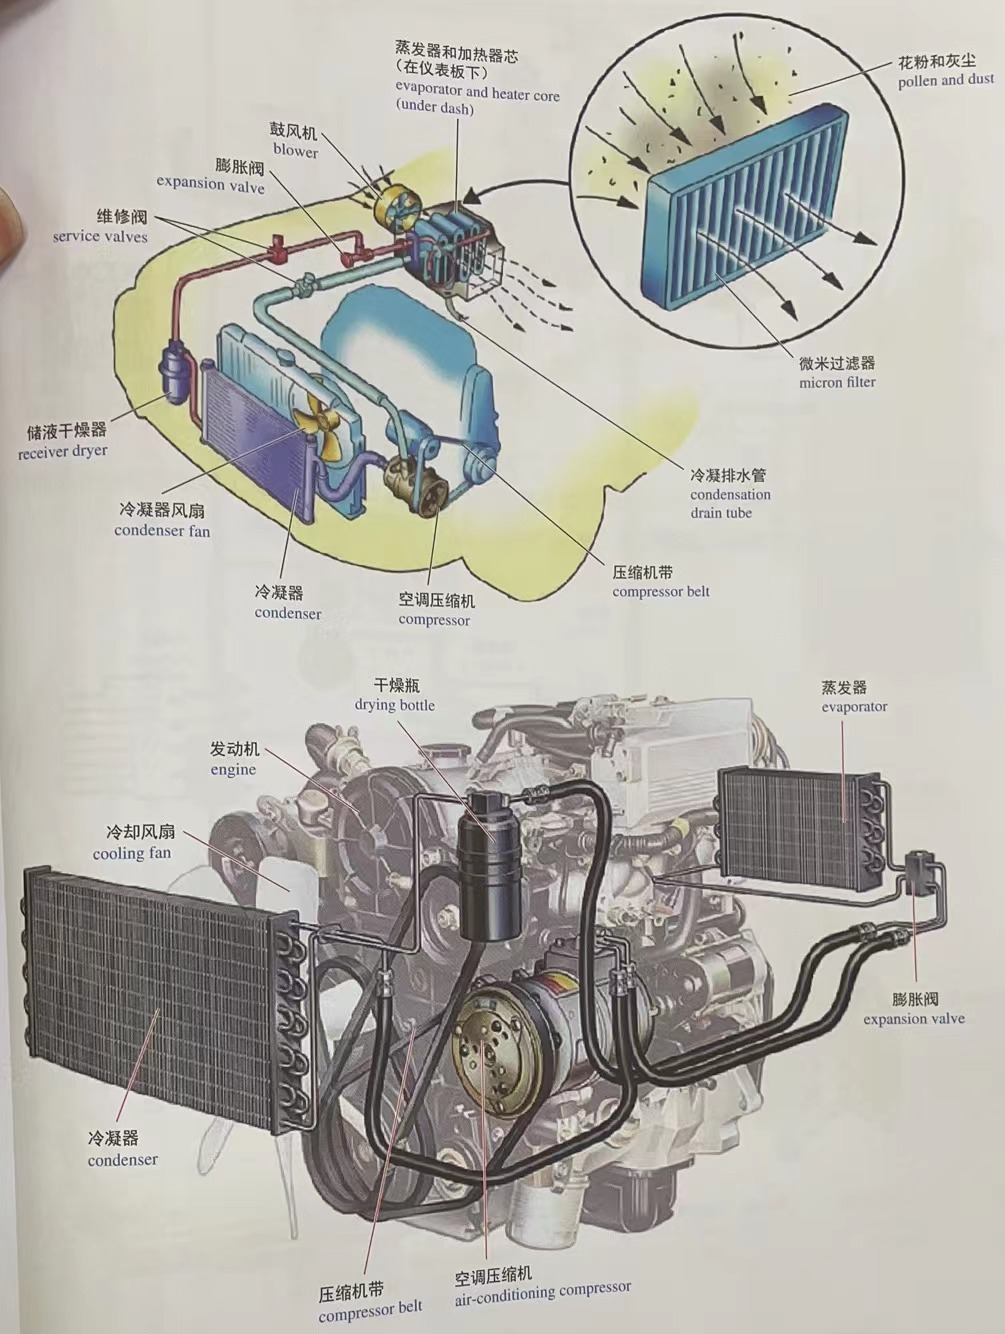
\includegraphics[width=0.5\textwidth]{5-19}
		\end{center}
	\subsubsection{电车空调}
		\begin{center}
			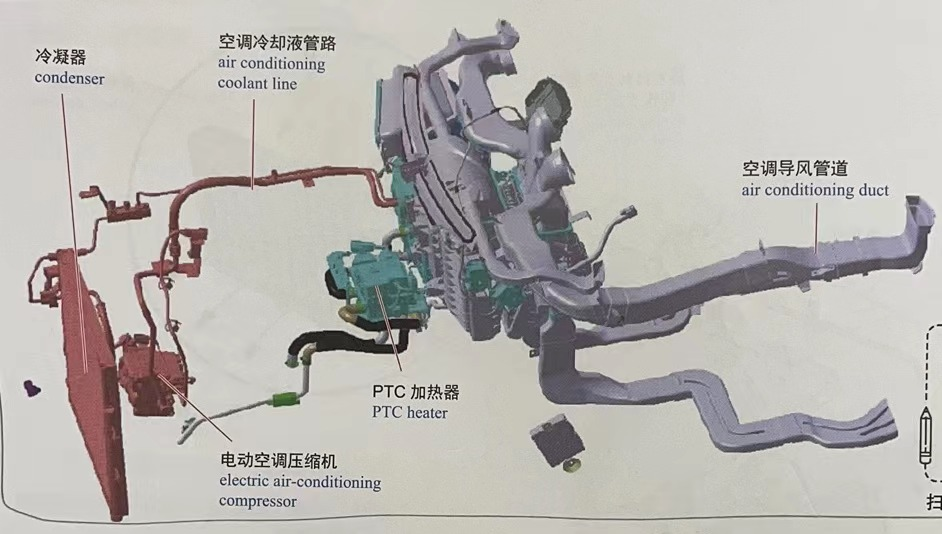
\includegraphics[width=0.5\textwidth]{5-20}
		\end{center}
	\subsubsection{制冷过程}
		压缩过程:压缩机将低温低压制冷器制成高温高压气体
		
		散热过程:冷凝器将高温高压气体冷凝成液体
		
		节流过程:膨胀阀使液体体积变大从而使压力和温度急剧下降
		
		吸热过程:蒸发器使液体蒸发,吸收周围热量
	\subsubsection{空调压缩机}
		\begin{figure}[htbp]
			\centering
			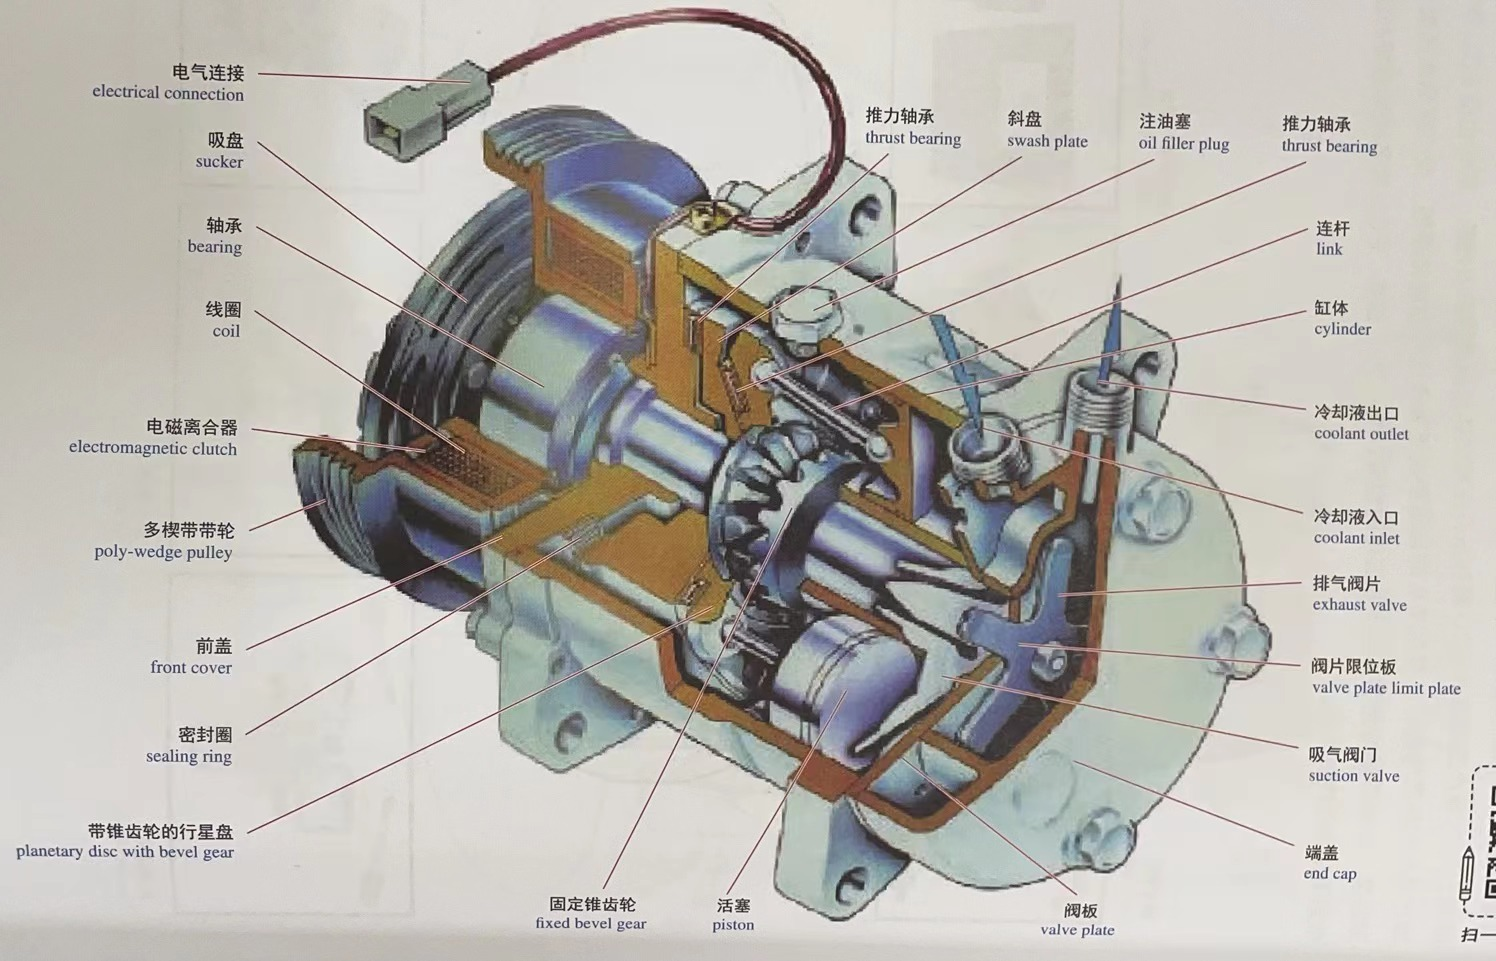
\includegraphics[width=0.5\textwidth]{5-21}
		\end{figure}

\subsection{车载信息娱乐系统IVI(in-vehicle infotainment)}
	整合了音响、导航、通信
	\begin{figure}[htbp]
		\centering
		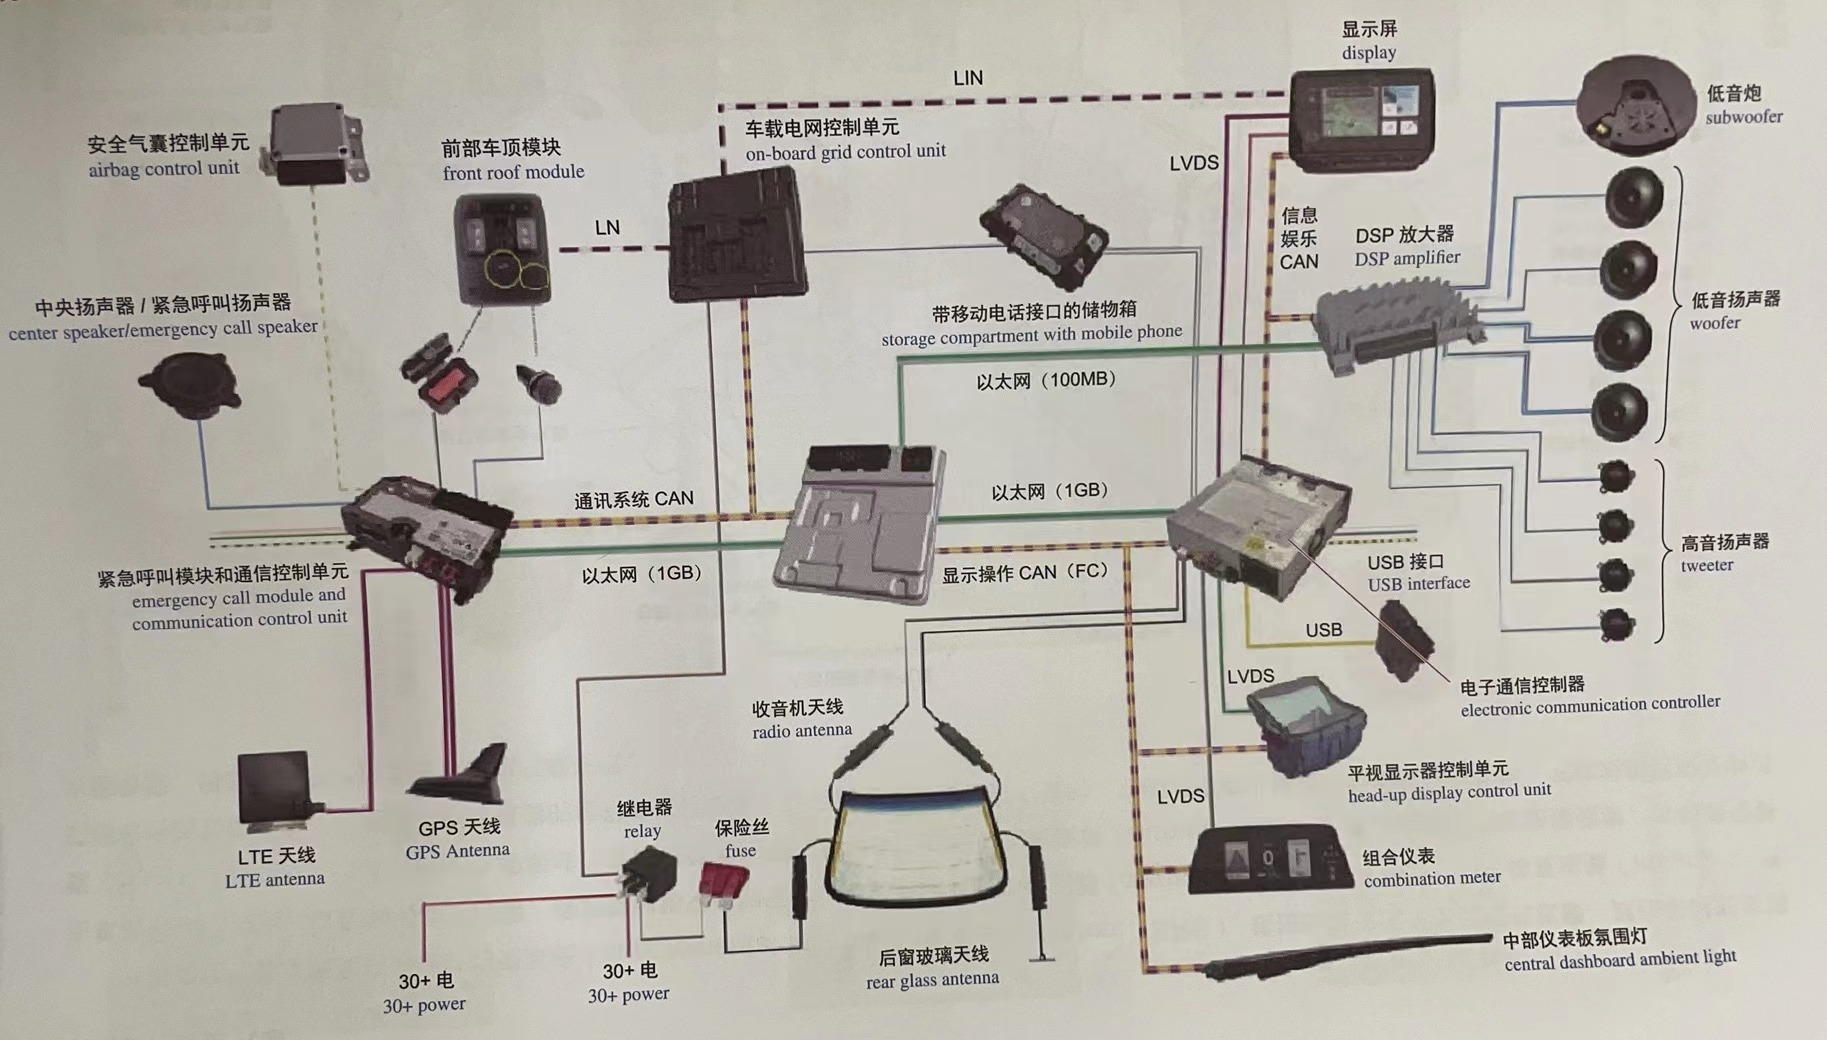
\includegraphics[width=0.5\textwidth]{5-22}
	\end{figure}
\subsection{安全气囊系统}
	又称辅助约束系统。一般有传感器、电控单元、气体发生器、气囊、续流器等组成。气体发生器和气囊一起构成气囊模块
	
	工作过程:传感器感受碰撞强度,发送信号到控制器,控制器判断是否打开气囊
	\begin{figure}[htbp]
		\centering
		\caption*{安全气囊分布}
		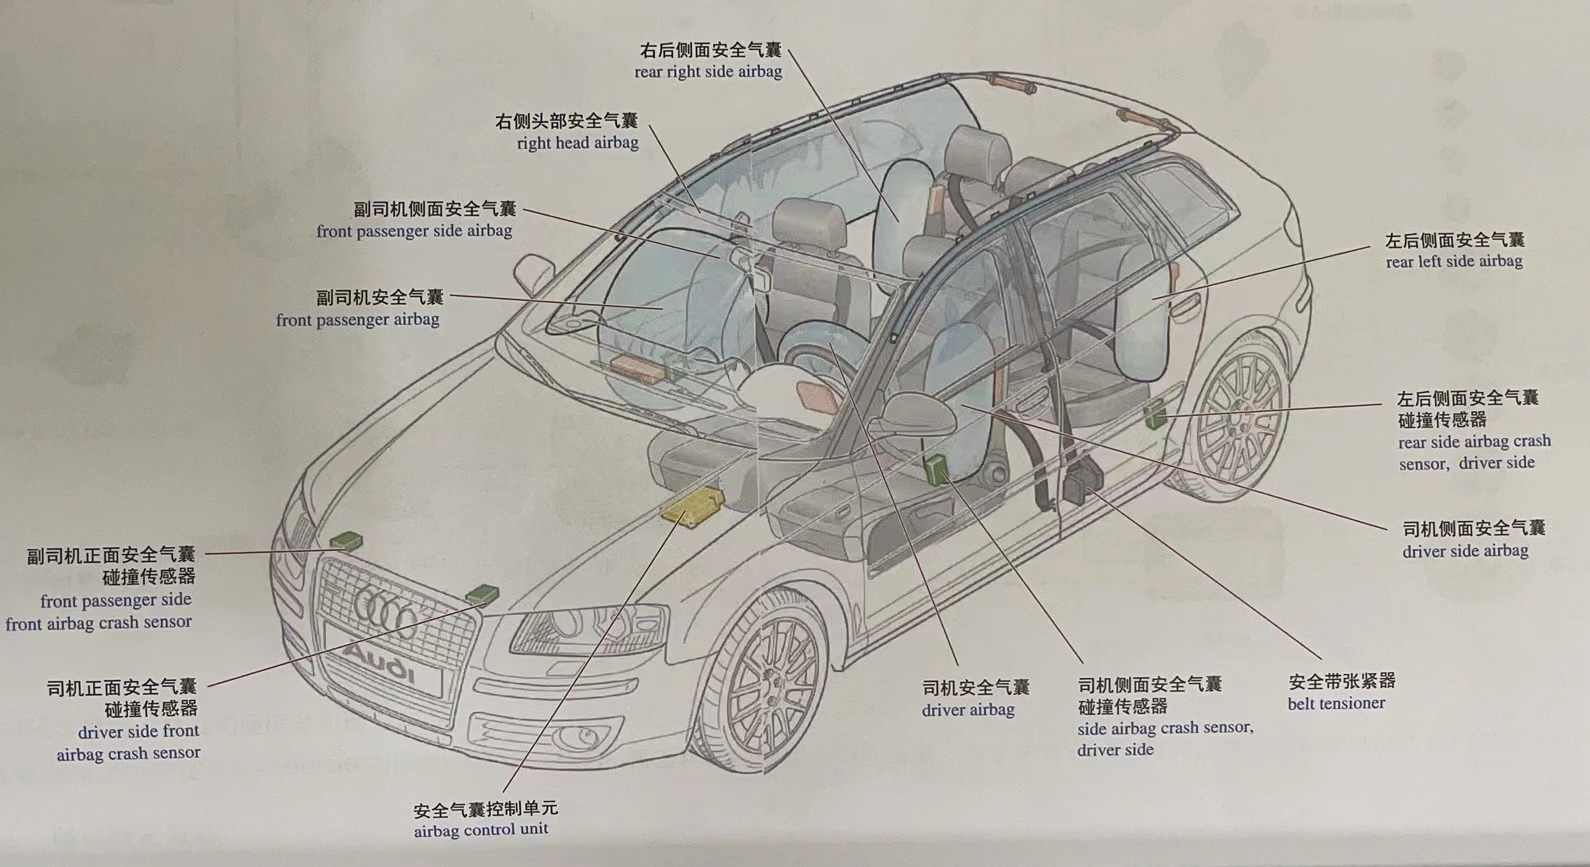
\includegraphics[width=0.5\textwidth]{5-23}
	\end{figure}
\subsection{防盗系统}
	分为发动机防盗系统IMMO(immobilization)、遥控门锁RKE(remote keyless entry)、无钥匙进入及启动系统PEPS(passive entry passive start)
	
	IMMO,RKE应用最广
\subsection{车声控制模块BCM}
	通过高速CAN总线与其他主要电子系统交互作用,通过LIN总线与次要的电气系统交互作用
	\begin{figure}[htbp]
		\centering
		\caption*{模块组成}
		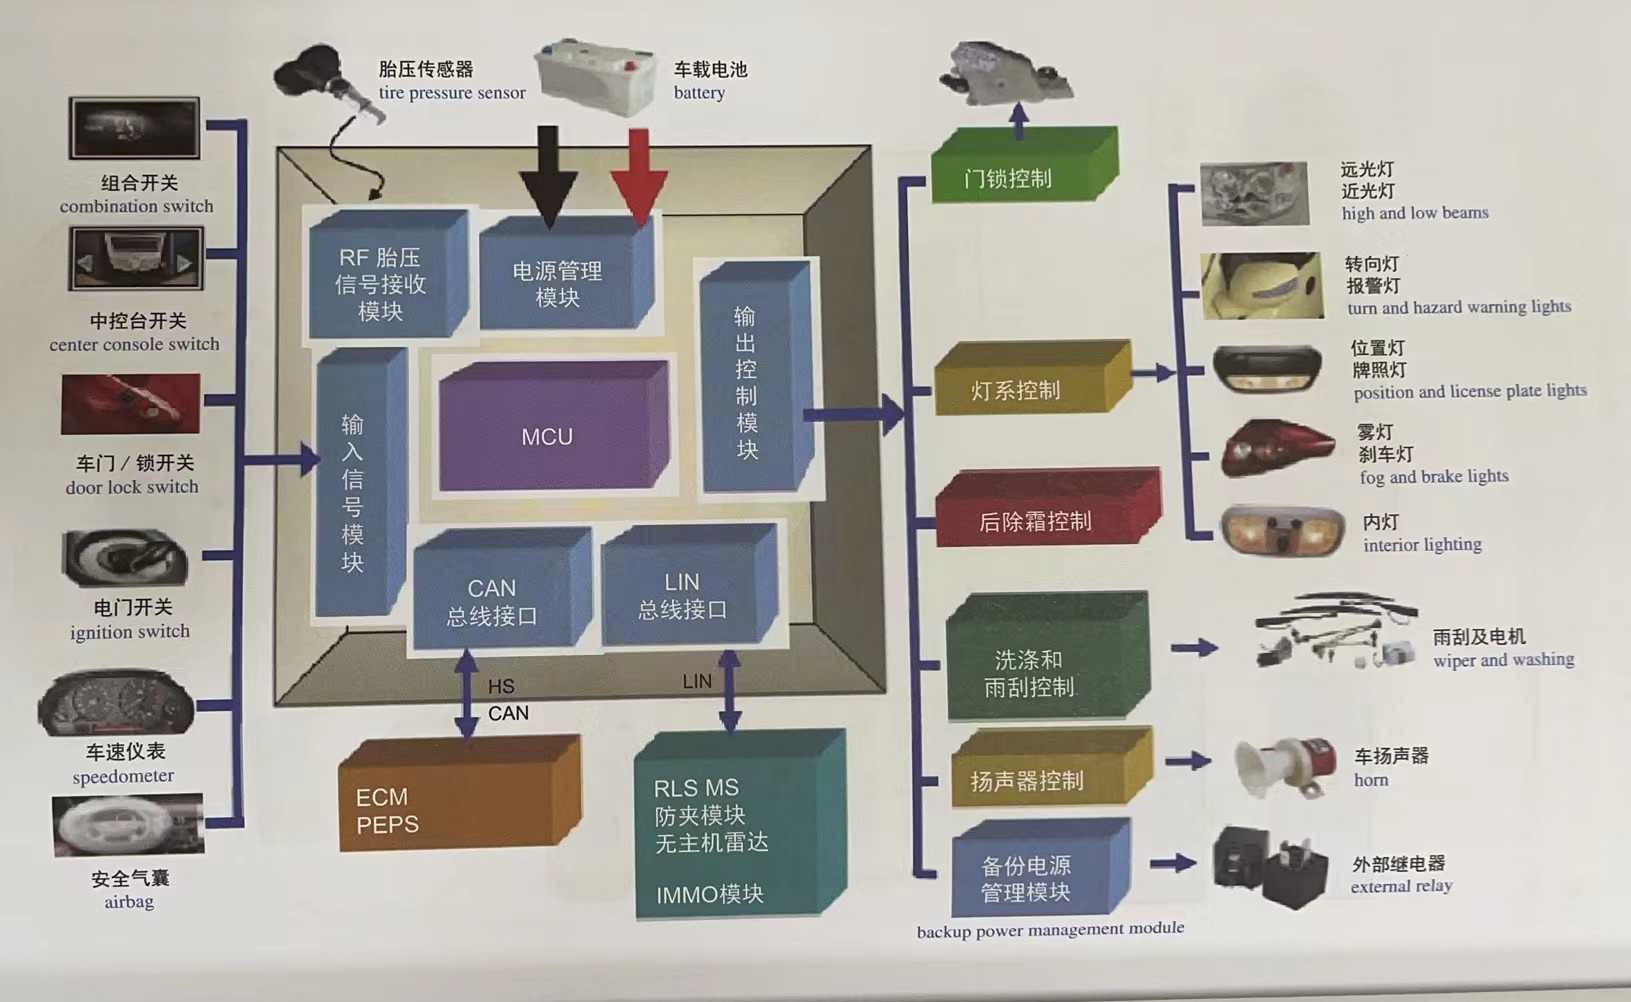
\includegraphics[width=0.5\textwidth]{5-24}
	\end{figure}
\subsection{车载网络}
	主流采用的总线有:局部互联协议LIN,控制器局域网CAN
	\subsubsection{CAN(controller area network)}
		双线系统,双线同时工作
	
		最大稳定传输率1Mbit/s
	\subsubsection{LIN(local interconnect network)}
		单线系统,每一次只交换一个控制单元的数据,各个LIN总线系统之间的数据交换是通过CAN总线实现的
		
		最大稳定传输率1-20kbit/s
\section{自动驾驶系统/高级辅助驾驶系统ADAS(advanced driver assistant systems)}
\subsection{分级表}
	\begin{figure}[htbp]
		\centering
		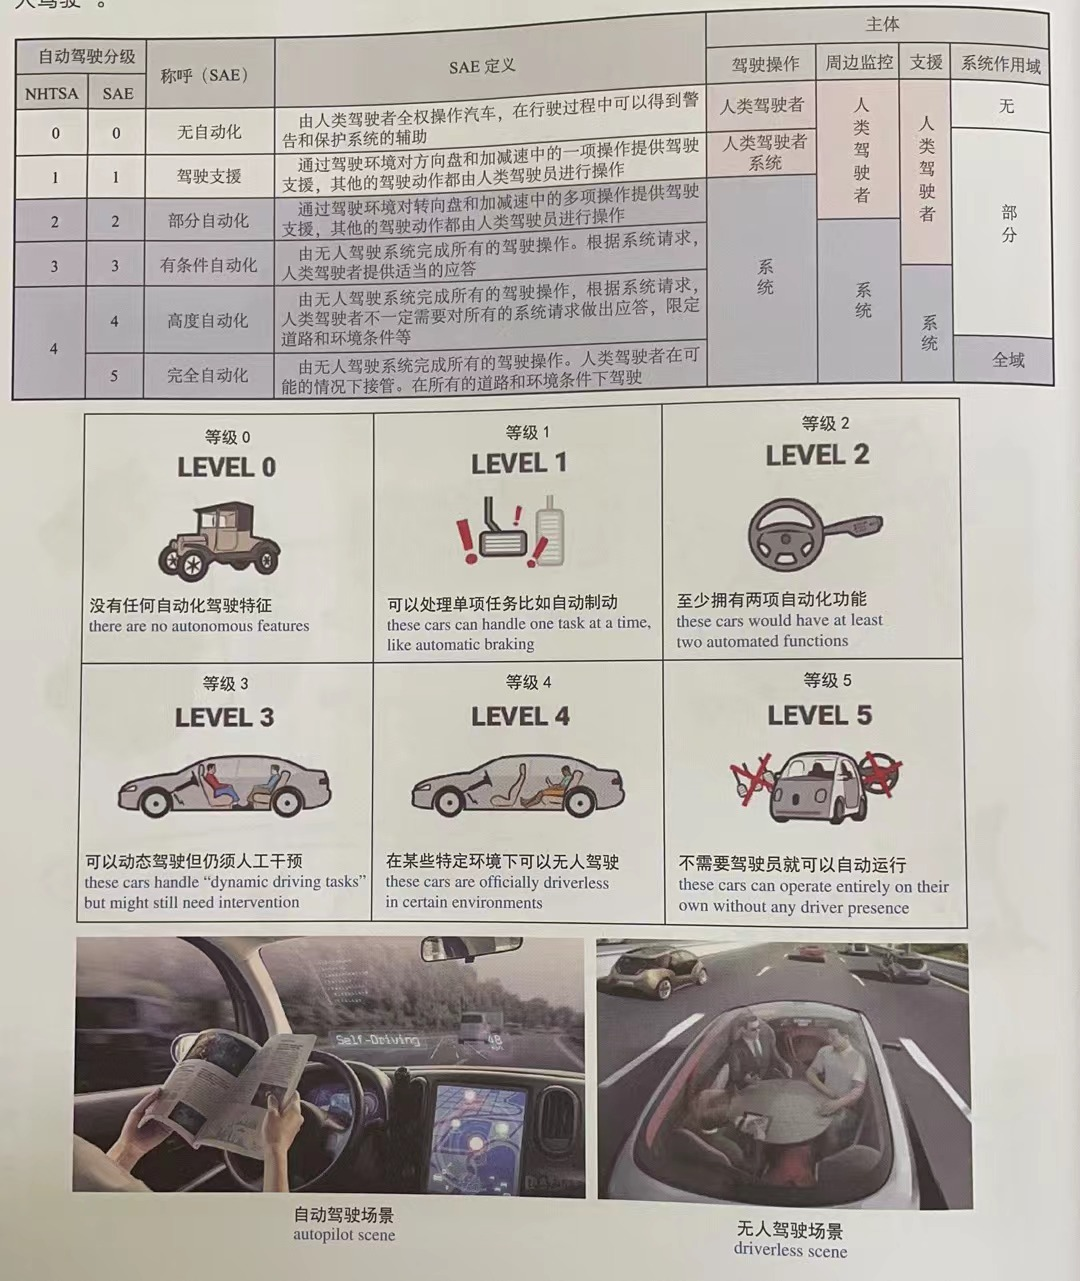
\includegraphics[width=0.5\textwidth]{5-25}
	\end{figure}
\subsection{系统组成}
	\begin{center}
		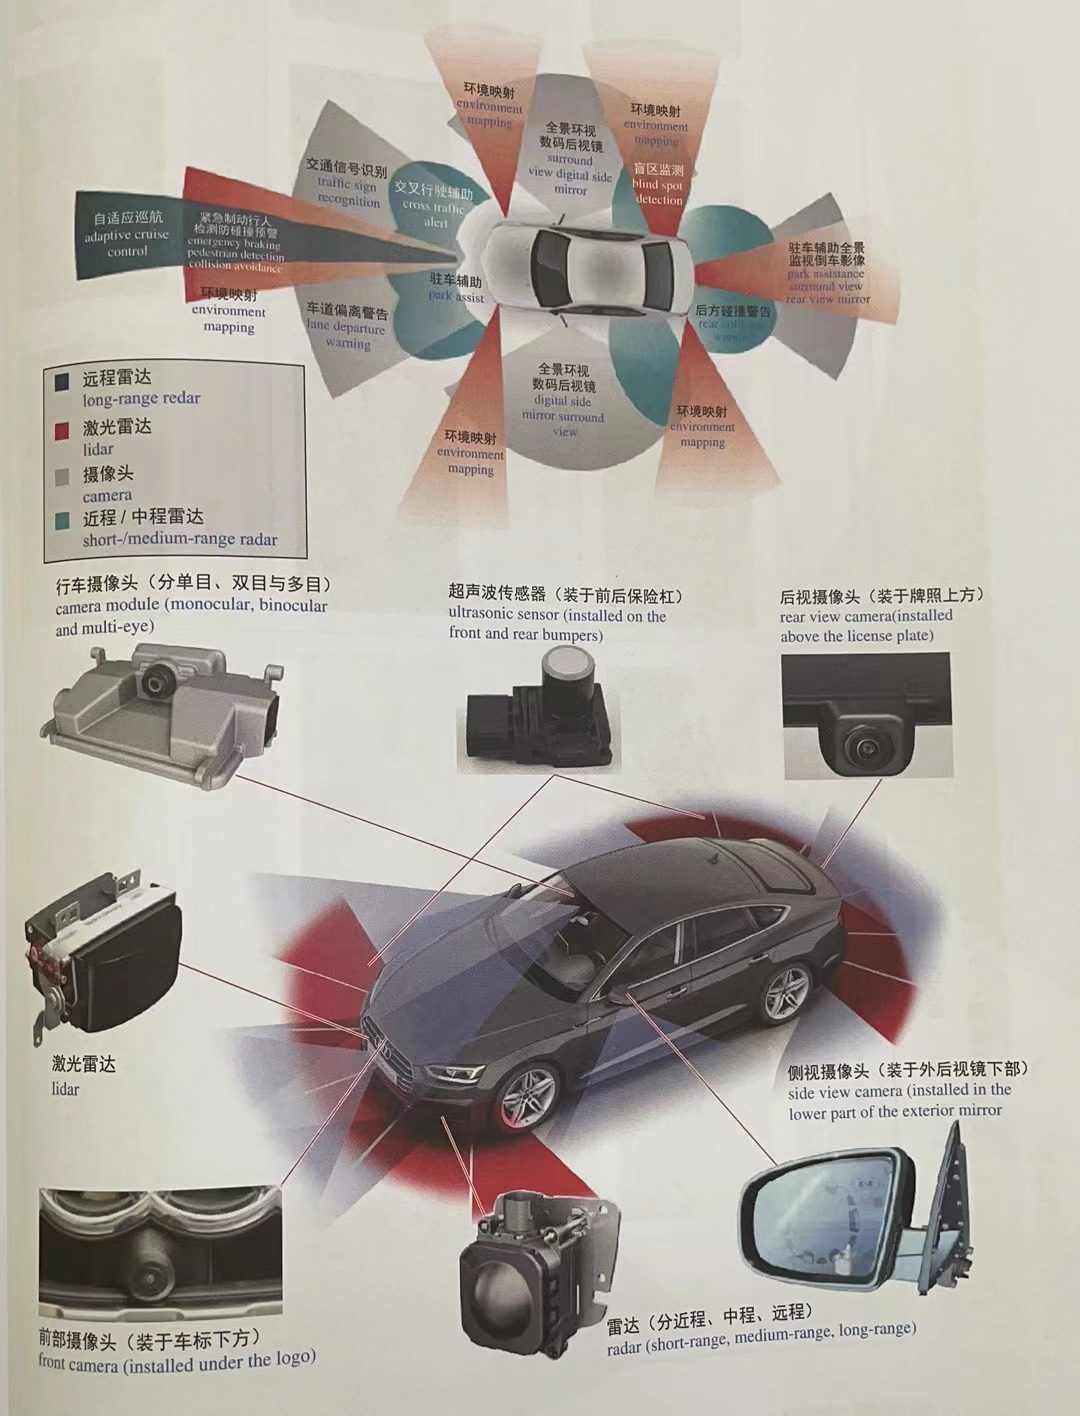
\includegraphics[width=0.5\textwidth]{5-26}
	\end{center}
\subsection{系统功能}
	\begin{figure}[htbp]
		\centering
		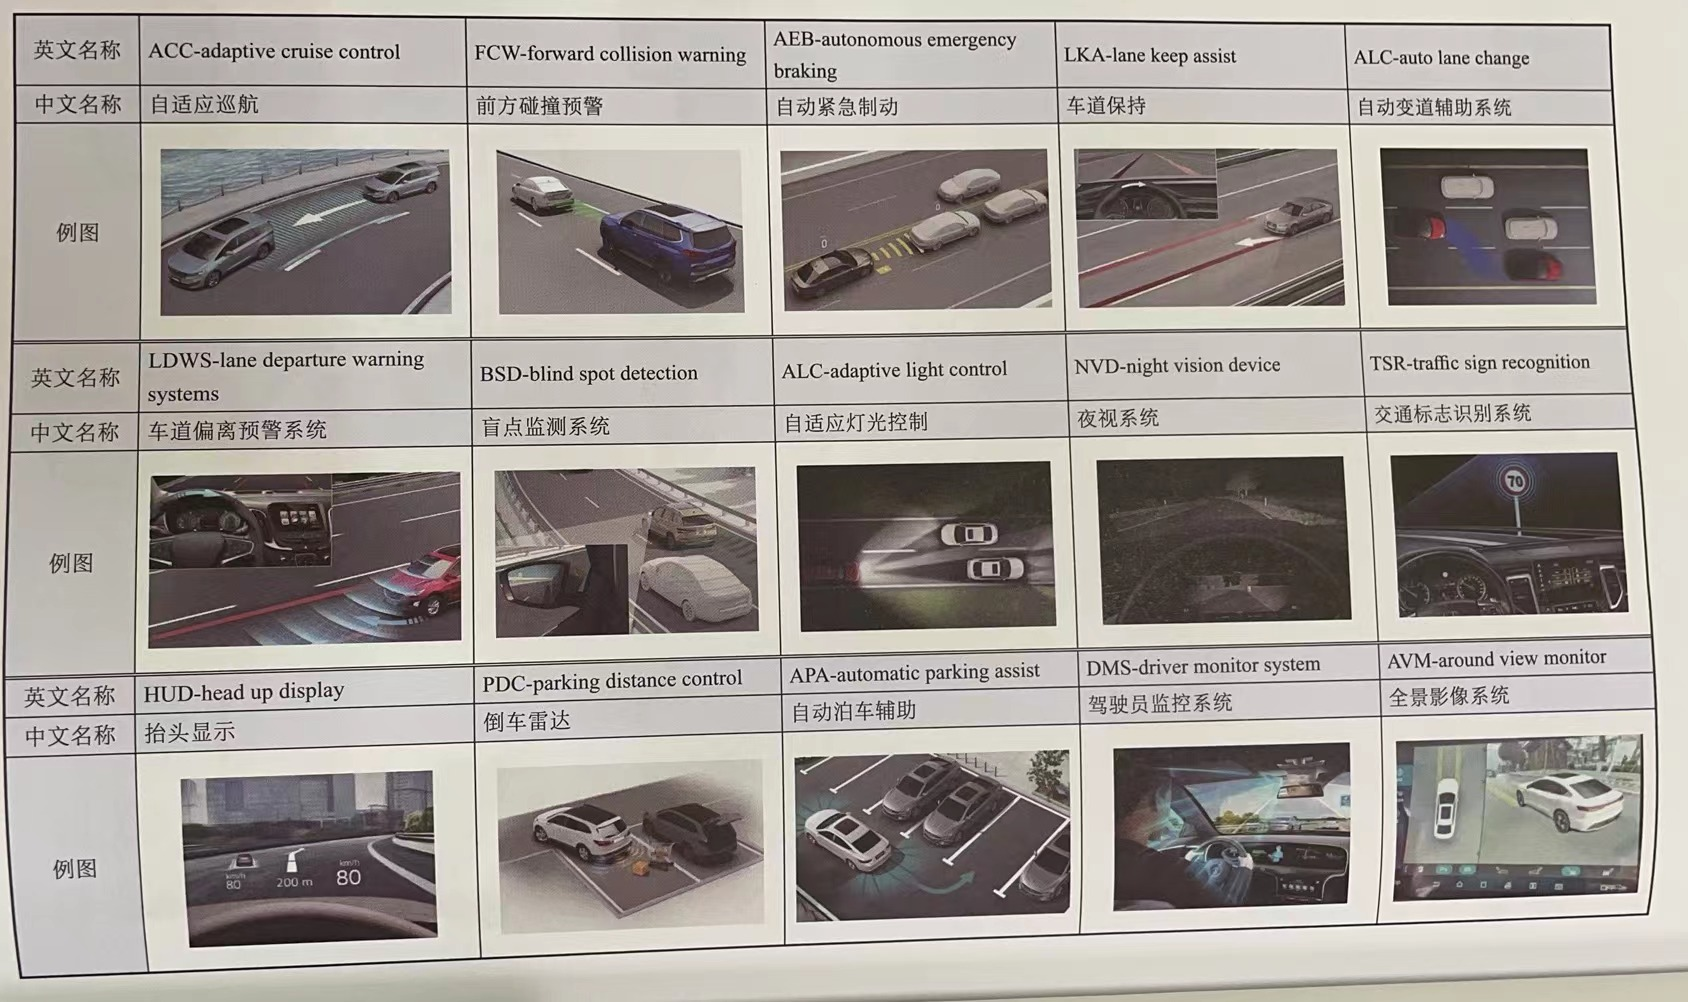
\includegraphics[width=0.5\textwidth]{5-27}
	\end{figure}
\end{document}
